%%%%%%%%%%%%%%%%%%%%%%%%%%%%%%%%%%%%%%%%%%%%%%%%%%%%%%%%%%%%%%%%%%%%%%%%%%%%%%%%
%  Zawartość: Główny plik szablonu pracy dyplomowej (magisterskiej/inżynierskiej). 
%  Opracował: Tomasz Kubik <tomasz.kubik@pwr.edu.pl>
%  Data: styczeń 2023
%  Wersja: 0.9
%  Wymagania: kompilator pdflatex
%%%%%%%%%%%%%%%%%%%%%%%%%%%%%%%%%%%%%%%%%%%%%%%%%%%%%%%%%%%%%%%%%%%%%%%%%%%%%%%%

\documentclass[a4paper,onecolumn,oneside,12pt,extrafontsizes]{memoir}
%  W celu przygotowania wydruku do archiwum można:
%  a) przygotować pdf, w którym dwie strony zostaną wstawione na jedną fizyczną stronę i taki dokument wydrukować dwustronnie (podejście zalecane)
%
%   Taki dokument można przygotować poprzez
%   - wydruk z Adobe Acrobat Reader z opcją "Wiele" - sekcja "Rozmiar i obsługa stron"
%   - wykorzystanie narzędzi psutils
%
%      Windows (zakładając, że w dystrybucji MiKTeX jest pakiet miktex-psutils-bin-x64-2.9):
%        "c:\Program Files\MiKTeX 2.9\miktex\bin\x64\pdf2ps.exe" Dyplom.pdf Dyplom.ps
%        "c:\Program Files\MiKTeX 2.9\miktex\bin\x64\psnup.exe" -2 Dyplom.ps Dyplom2.ps
%        "c:\Program Files\MiKTeX 2.9\miktex\bin\x64\ps2pdf.exe" Dyplom2.ps Dyplom2.pdf
%        Del Dyplom2.ps Dyplom.ps
%
%     Linux:
%        pdf2ps Dyplom.pdf - | psnup -2 | ps2pdf - Dyplom2.pdf
%
%  b) przekomplilować dokument zmniejszając czcionkę (podejście niezalecane, bo zmienia formatowanie dokumentu)
%
%    Do tego wystarczy posłużyć się poniższymi komendami (zamiast documentclass z pierwszej linijki):
%   \documentclass[a4paper,onecolumn,twoside,10pt]{memoir} 
%   \renewcommand{\normalsize}{\fontsize{8pt}{10pt}\selectfont}

%\usepackage[cp1250]{inputenc} % Proszę zostawić, jeśli kodowanie edytowanych plików to cp1250 
\usepackage[utf8]{inputenc} % Proszę użyć zamiast powyższego, jeśli kodowanie edytowanych plików to UTF8
\usepackage[T1]{fontenc}
\usepackage[english,polish]{babel} % Tutaj ważna jest kolejność atrybutów (dla pracy po polsku polish powinno być na końcu)
%\DisemulatePackage{setspace}
\usepackage{setspace}
\usepackage{color,calc}
%\usepackage{soul} % pakiet z komendami do podkreślania, przekreślania, podświetlania tekstu (raczej niepotrzebny)
\usepackage{ebgaramond} % pakiet z czcionkami garamond, potrzebny tylko do strony tytułowej, musi wystąpić przed pakietem tgtermes

%% Aby uzyskać polskie literki w pdfie (a nie zlepki) korzystamy z pakietu czcionek tgterms. 
%% W pakiecie tym są zdefiniowane klony czcionek Times o kształtach: normalny, pogrubiony, italic, italic pogrubiony.
%% W pakiecie tym brakuje czcionki o kształcie: slanted (podobny do italic). 
%% Jeśli w dokumencie gdzieś zostanie zastosowana czcionka slanted (np. po użyciu komendy \textsl{}), to
%% latex dokona podstawienia na czcionkę standardową i zgłosi to w ostrzeżeniu (warningu).
%% Ponadto tgtermes to czcionka do tekstu. Wszelkie matematyczne wzory będą sformatowane domyślną czcionką do wzorów.
%% Jeśli wzory mają być sformatowane z wykorzystaniem innych czcionek, trzeba to jawnie zadeklarować.

%% Po zainstalowaniu pakietu tgtermes może będzie trzeba zauktualizować informacje 
%% o dostępnych fontach oraz mapy. Można to zrobić z konsoli (jako administrator)
%% initexmf --admin --update-fndb
%% initexmf --admin --mkmaps

\usepackage{tgtermes}   
\renewcommand*\ttdefault{txtt}


%%%%%%%%%%%%%%%%%%%%%%%%%%%%%%%%%%%%%%%%%%%%%%%%%%%%%%%%%%%%%%%%%%%%%%%%%%%%%%%%
%% Ustawienia odpowiedzialne za sposób łamania dokumentu
%% i ułożenie elementów pływających
%%%%%%%%%%%%%%%%%%%%%%%%%%%%%%%%%%%%%%%%%%%%%%%%%%%%%%%%%%%%%%%%%%%%%%%%%%%%%%%%
%\hyphenpenalty=10000		% nie dziel wyrazów zbyt często
\clubpenalty=10000      % kara za sierotki
\widowpenalty=10000     % nie pozostawiaj wdów
%\brokenpenalty=10000		% nie dziel wyrazów między stronami - trzeba było wyłączyć, bo nie łamały się linie w lstlisting
%\exhyphenpenalty=999999		% nie dziel słów z myślnikiem - trzeba było wyłączyć, bo nie łamały się linie w lstlisting
\righthyphenmin=3			  % dziel minimum 3 litery

%\tolerance=4500
%\pretolerance=250
%\hfuzz=1.5pt
%\hbadness=1450

\renewcommand{\topfraction}{0.95}
\renewcommand{\bottomfraction}{0.95}
\renewcommand{\textfraction}{0.05}
\renewcommand{\floatpagefraction}{0.35}

%%%%%%%%%%%%%%%%%%%%%%%%%%%%%%%%%%%%%%%%%%%%%%%%%%%%%%%%%%%%%%%%%%%%%%%%%%%%%%%%
%%  Ustawienia rozmiarów: tekstu, nagłówka i stopki, marginesów
%%  dla dokumentów klasy memoir 
%%%%%%%%%%%%%%%%%%%%%%%%%%%%%%%%%%%%%%%%%%%%%%%%%%%%%%%%%%%%%%%%%%%%%%%%%%%%%%%%
\setlength{\headsep}{10pt} 
\setlength{\headheight}{13.6pt} % wartość baselineskip dla czcionki 11pt tj. \small wynosi 13.6pt
\setlength{\footskip}{\headsep+\headheight}
\setlength{\uppermargin}{\headheight+\headsep+1cm}
\setlength{\textheight}{\paperheight-\uppermargin-\footskip-1.5cm}
\setlength{\textwidth}{\paperwidth-5cm}
\setlength{\spinemargin}{2.5cm}
\setlength{\foremargin}{2.5cm}
\setlength{\marginparsep}{2mm}
\setlength{\marginparwidth}{2.3mm}
%\settrimmedsize{297mm}{210mm}{*}
%\settrims{0mm}{0mm}	
\checkandfixthelayout[fixed] % konieczne, aby się dobrze wszystko poustawiało
%%%%%%%%%%%%%%%%%%%%%%%%%%%%%%%%%%%%%%%%%%%%%%%%%%%%%%%%%%%%%%%%%%%%%%%%%%%%%%%%
%%  Ustawienia odległości linii, wcięć, odstępów
%%%%%%%%%%%%%%%%%%%%%%%%%%%%%%%%%%%%%%%%%%%%%%%%%%%%%%%%%%%%%%%%%%%%%%%%%%%%%%%%
\linespread{1}
%\linespread{1.241}
\setlength{\parindent}{14.5pt}


\usepackage{multicol} % pakiet umożliwiający stworzenie wielokolumnowego tekstu
\usepackage{multirow}
%%%%%%%%%%%%%%%%%%%%%%%%%%%%%%%%%%%%%%%%%%%%%%%%%%%%%%%%%%%%%%%%%%%%%%%%%%%%%%%%
%% Pakiety do formatowania tabel
%%%%%%%%%%%%%%%%%%%%%%%%%%%%%%%%%%%%%%%%%%%%%%%%%%%%%%%%%%%%%%%%%%%%%%%%%%%%%%%%
\usepackage{tabularx}
% Proszę używać tylko tabularx. Innych pakietów proszę nie stosować !!!
% Dokument na pewno da się zredagować bez ich użycia.
%\usepackage{longtable}
%\usepackage{ltxtable}
%\usepackage{tabulary}

%%%%%%%%%%%%%%%%%%%%%%%%%%%%%%%%%%%%%%%%%%%%%%%%%%%%%%%%%%%%%%%%%%%%%%%%%%%%%%%%
%% Pakiet do wstawiania fragmentów kodu
%%%%%%%%%%%%%%%%%%%%%%%%%%%%%%%%%%%%%%%%%%%%%%%%%%%%%%%%%%%%%%%%%%%%%%%%%%%%%%%%
\usepackage{listings} 
\usepackage{xpatch}
\makeatletter
\xpatchcmd\l@lstlisting{1.5em}{0em}{}{}
\makeatother
% Pakiet dostarcza otoczenia lstlisting. Jest ono wysoce konfigurowalne. 
% Konfigurować można indywidualnie każdy z listingów lub globalnie, w poleceniu \lstset{}.

% Zalecane jest, by kod źródłowy był wyprowadzany z użyciem czcionki maszynowej \ttfamily
% Ponieważ kod źródłowy, nawet po obcięciu do interesujących fragmentów, bywa obszerny, należy zmniejszyć czcionkę.
% Zalecane jest \small (dla krótkich fragmentów) oraz \footnotesize (dla dłuższych fragmentów).

% Ponadto podczas konfiguracji można zadeklarować sposób numerowania linii. Numerowanie linii zalecane jest jednak 
% tylko w przypadkach, gdy w redagowanym tekście znajdują się jakieś odwołania do konkretnych linii.
% Jeśli takich odwołań nie ma, numerowanie linii jest zbędne. Proszę wtedy go nie stosować.
% Przy włączaniu numerowania linii należy zwrócić uwagę na to, gdzie pojawią się te numery.
% Bez zmiany dodatkowych parametrów pojawiają się one na marginesie strony (co jest niepożądane).

\lstset{
  basicstyle=\small\ttfamily, % lub basicstyle=\footnotesize\ttfamily
  %%columns=fullflexible,
	%%showstringspaces=false,
	%%showspaces=false,
  breaklines=true,
  postbreak=\mbox{\textcolor{red}{$\hookrightarrow$}\space}, 
  %%numbers=left,  % ta i poniższe linie dotyczą ustawienia numerowania i sposobu jego wyprowadzania
  %%firstnumber=1, 
  %%numberfirstline=true, 
	%%xleftmargin=17pt,
  %%framexleftmargin=17pt,
  %%framexrightmargin=5pt,
  %%framexbottommargin=4pt,
	belowskip=.5\baselineskip,
	literate={\_}{{\_\allowbreak}}1 % ta deklaracja przydaje się, jeśli na listingu mają być łamane nazwy zawierające podkreślniki
}

% Jeśli edytowany plik nie jest w kodowaniu cp1250, to jest problem z polskimi znakami występującymi we wstawianym kodzie.
% Dlatego podczas pracy na plikach w kodowaniu UTF8 trzeba zadeklarować mapowanie jak niżej (wystarczy odmarkować).
% Niestety, jak się zastosuje to mapowanie mogą pojawić się problemy z podświetlaniem składni (patrz dalej).
\lstset{literate=%-
{ą}{{\k{a}}}1 {ć}{{\'c}}1 {ę}{{\k{e}}}1 {ł}{{\l{}}}1 {ń}{{\'n}}1 {ó}{{\'o}}1 {ś}{{\'s}}1 {ż}{{\.z}}1 {ź}{{\'z}}1 {Ą}{{\k{A}}}1 {Ć}{{\'C}}1 {Ę}{{\k{E}}}1 {Ł}{{\L{}}}1 {Ń}{{\'N}}1 {Ó}{{\'O}}1 {Ś}{{\'S}}1 {Ż}{{\.Z}}1 {Ź}{{\'Z}}1 
    {Ö}{{\"O}}1
    {Ä}{{\"A}}1
    {Ü}{{\"U}}1
    {ß}{{\ss}}1
    {ü}{{\"u}}1
    {ä}{{\"a}}1
    {ö}{{\"o}}1
    {~}{{\textasciitilde}}1
		{—}{{{\textemdash} }}1
}%{\ \ }{{\ }}1}


%% lstlisting pozwala na ostylowania podświetlania składni wybranych języków.
%% Działa to na zasadzie zdefiniowania słów kluczowych oraz sposobu ich wyświetlania.
%% Ponieważ jest to prosty mechanizm, czasem trudno osiągnąć takie efekty, jakie dają narzędzia IDE. 
%% Jednak w większości przypadku osiągane rezutlaty są zadowalające.


%% lstlisting obsługuje domyślnie kilka najpopularniejszych języków.
\lstloadlanguages{% Check Dokumentation for further languages ...
%%C,
%%C++,
csh
%%Java
}
%% Inne języki muszą być dodefiniowane. Poniżej podano przykłady definicji języków i styli.

%%\definecolor{lightgray}{rgb}{.9,.9,.9}
%%\definecolor{darkgray}{rgb}{.4,.4,.4}
%%\definecolor{purple}{rgb}{0.65, 0.12, 0.82}
%%\definecolor{javared}{rgb}{0.6,0,0} % for strings
%%\definecolor{javagreen}{rgb}{0.25,0.5,0.35} % comments
%%\definecolor{javapurple}{rgb}{0.5,0,0.35} % keywords
%%\definecolor{javadocblue}{rgb}{0.25,0.35,0.75} % javadoc
 %%
%%\lstdefinelanguage{JavaScript}{ 
	%%keywords={typeof, new, true, false, catch, function, return, null, catch, switch, var, if, in, while, do, else, case, break},
	%%keywordstyle=\color{blue}\bfseries,
	%%ndkeywords={class, export, boolean, throw, implements, import, this},
	%%ndkeywordstyle=\color{darkgray}\bfseries,
	%%identifierstyle=\color{black},
	%%sensitive=false,
	%%comment=[l]{//},
	%%morecomment=[s]{/*}{*/},
	%%commentstyle=\color{purple}\ttfamily,
	%%stringstyle=\color{red}\ttfamily,
	%%morestring=[b]',
	%%morestring=[b]"
%%}
%%\lstdefinestyle{JavaScriptStyle}{
	%%language=JavaScript,
	%%commentstyle=\color{javagreen}, % niestety, jeśli w linii komentarza pojawią się słowa kluczowe, to zostaną pokolorowane
	%%backgroundcolor=,%\color{lightgray}, % można ustwić kolor tła, ale jest to niezalecane
	%%extendedchars=true,
	%%basicstyle=\footnotesize\ttfamily,
	%%showstringspaces=false,
	%%showspaces=false,
	%%numbers=none,%left,
	%%numberstyle=\footnotesize,
	%%numbersep=9pt,
	%%tabsize=2,
	%%breaklines=true,
	%%showtabs=false,
	%%captionpos=t
%%}
%%
%%\lstdefinestyle{JavaStyle}{
%%basicstyle=\footnotesize\ttfamily,
%%keywordstyle=\color{javapurple}\bfseries,
%%stringstyle=\color{javared},
%%commentstyle=\color{javagreen},
%%morecomment=[s][\color{javadocblue}]{/**}{*/},
%%numbers=none,%left,
%%numberstyle=\tiny\color{black},
%%stepnumber=2,
%%numbersep=10pt,
%%tabsize=4,
%%showspaces=false,
%%showstringspaces=false,
%%captionpos=t
%%}
%%
%%\definecolor{pblue}{rgb}{0.13,0.13,1}
%%\definecolor{pgreen}{rgb}{0,0.5,0}
%%\definecolor{pred}{rgb}{0.9,0,0}
%%\definecolor{pgrey}{rgb}{0.46,0.45,0.48}
%%\definecolor{dark-grey}{rgb}{0.4,0.4,0.4}
%%% styl json
%%\newcommand\JSONnumbervaluestyle{\color{blue}}
%%\newcommand\JSONstringvaluestyle{\color{red}}
%%
%%\newif\ifcolonfoundonthisline
%%
%%\makeatletter
%%
%%\lstdefinestyle{json-style}  
%%{
	%%showstringspaces    = false,
	%%keywords            = {false,true},
	%%alsoletter          = 0123456789.,
	%%morestring          = [s]{"}{"},
	%%stringstyle         = \ifcolonfoundonthisline\JSONstringvaluestyle\fi,
	%%MoreSelectCharTable =%
	%%\lst@DefSaveDef{`:}\colon@json{\processColon@json},
	%%basicstyle          = \footnotesize\ttfamily,
	%%keywordstyle        = \ttfamily\bfseries,
	%%numbers				= left, % zakomentować, jeśli numeracja linii jest niepotrzebna
	%%numberstyle={\footnotesize\ttfamily\color{dark-grey}},
	%%xleftmargin			= 2em % zakomentować, jeśli numeracja linii jest niepotrzebna
%%}
%%
%%\newcommand\processColon@json{%
	%%\colon@json%
	%%\ifnum\lst@mode=\lst@Pmode%
	%%\global\colonfoundonthislinetrue%
	%%\fi
%%}
%%
%%\lst@AddToHook{Output}{%
	%%\ifcolonfoundonthisline%
	%%\ifnum\lst@mode=\lst@Pmode%
	%%\def\lst@thestyle{\JSONnumbervaluestyle}%
	%%\fi
	%%\fi
	%%\lsthk@DetectKeywords% 
%%}
%%
%%\lst@AddToHook{EOL}%
%%{\global\colonfoundonthislinefalse}
%%
%%\makeatother

\definecolor{red}{rgb}{0.6,0,0} % for strings
\definecolor{blue}{rgb}{0,0,0.6}
\definecolor{green}{rgb}{0,0.8,0}
\definecolor{cyan}{rgb}{0.0,0.6,0.6}

%%\lstdefinestyle{sqlstyle}{
%%language=SQL,
%%basicstyle=\footnotesize\ttfamily, 
%%numbers=left, 
%%numberstyle=\tiny, 
%%numbersep=5pt, 
%%tabsize=2, 
%%extendedchars=true, 
%%breaklines=true, 
%%showspaces=false, 
%%showtabs=true, 
%%xleftmargin=17pt,
%%framexleftmargin=17pt,
%%framexrightmargin=5pt,
%%framexbottommargin=4pt,
%%keywordstyle=\color{blue}, 
%%commentstyle=\color{green}, 
%%stringstyle=\color{red}, 
%%}

\lstdefinestyle{sharpcstyle}{
language=[Sharp]C,
basicstyle=\ttfamily\footnotesize, 
%numbers=left, 
%numberstyle=\tiny, 
%numbersep=5pt, 
tabsize=2, 
extendedchars=true, 
breaklines=true, 
showspaces=false, 
showtabs=true, 
%xleftmargin=17pt,
%framexleftmargin=17pt,
%framexrightmargin=5pt,
%framexbottommargin=4pt,
morecomment=[l]{//}, %use comment-line-style!
morecomment=[s]{/*}{*/}, %for multiline comments
showstringspaces=false, 
morekeywords={  abstract, event, new, struct,
                as, explicit, null, switch,
                base, extern, object, this,
                bool, false, operator, throw,
                break, finally, out, true,
                byte, fixed, override, try,
                case, float, params, typeof,
                catch, for, private, uint,
                char, foreach, protected, ulong,
                checked, goto, public, unchecked,
                class, if, readonly, unsafe,
                const, implicit, ref, ushort,
                continue, in, return, using,
                decimal, int, sbyte, virtual,
                default, interface, sealed, volatile,
                delegate, internal, short, void,
                do, is, sizeof, while,
                double, lock, stackalloc,
                else, long, static,
                enum, namespace, string},
keywordstyle=\color{blue},
%identifierstyle=\color{red},
stringstyle=\color{red}, 
commentstyle=\color{green},
}

\definecolor{base0}{RGB}{131,148,150}
\definecolor{base01}{RGB}{88,110,117}
\definecolor{base2}{RGB}{238,232,213}
\definecolor{sgreen}{RGB}{133,153,0}
\definecolor{sblue}{RGB}{38,138,210}
\definecolor{scyan}{RGB}{42,161,151}
\definecolor{smagenta}{RGB}{211,54,130}


\newcommand\digitstyle{\color{smagenta}}
\newcommand\symbolstyle{\color{base01}}
\makeatletter
\newcommand{\ProcessDigit}[1]
{%
  \ifnum\lst@mode=\lst@Pmode\relax%
   {\digitstyle #1}%
  \else
    #1%
  \fi
}

\makeatother




%%%%%%%%%%%%%%%%%%%%%%%%%%%%%%%%%%%%%%%%%%%%%%%%%%%%%%%%%%%%%%%%%%%%%%%%%%%%%%%%
%%  Pakiety i komendy zastosowane tylko do zamieszczenia informacji o użytych komendach i fontach w tym szablonie.
%%  Normalnie nie są one potrzebne. Proszę poniższe deklaracje zamarkować podczas redakcji pracy !!!!
%%%%%%%%%%%%%%%%%%%%%%%%%%%%%%%%%%%%%%%%%%%%%%%%%%%%%%%%%%%%%%%%%%%%%%%%%%%%%%%%
%%%\usepackage{memlays}     % extra layout diagrams, zastosowane w szblonie do 'debuggowania', używa pakietu layouts
%%%%\usepackage{layouts}
%%%\usepackage{printlen} % pakiet do wyświetlania wartości zdefiniowanych długości, stosowany do 'debuggowania'
%%%\usepackage{enumitem} % pakiet do numerowania 1.1 1.2 w sekcji enumrate
%%%\uselengthunit{pt}
%%%\makeatletter
%%%\newcommand{\showFontSize}{\f@size pt} % makro wypisujące wielkość bieżącej czcionki
%%%\makeatother
% do pokazania ramek można byłoby użyć:
%\usepackage{showframe} 

%%%%%%%%%%%%%%%%%%%%%%%%%%%%%%%%%%%%%%%%%%%%%%%%%%%%%%%%%%%%%%%%%%%%%%%%%%%%%%%%
%%  Formatowanie list wyliczeniowych, wypunktowań i własnych otoczeń
%%%%%%%%%%%%%%%%%%%%%%%%%%%%%%%%%%%%%%%%%%%%%%%%%%%%%%%%%%%%%%%%%%%%%%%%%%%%%%%%

% Domyślnie wypunktowania mają zadeklarowane znaki, które nie występują w tgtermes
% Aby latex nie podstawiał w ich miejsca znaków z czcionki standardowej można zrobić podstawienie:
%    \DeclareTextCommandDefault{\textbullet}{\ensuremath{\bullet}}
%    \DeclareTextCommandDefault{\textasteriskcentered}{\ensuremath{\ast}}
%    \DeclareTextCommandDefault{\textperiodcentered}{\ensuremath{\cdot}}
% Jednak jeszcze lepszym pomysłem jest zdefiniowanie otoczeń z wykorzystaniem enumitem
\usepackage{enumitem} % pakiet pozwalający zarządzać formatowaniem list wyliczeniowych
\setlist{noitemsep,topsep=4pt,parsep=0pt,partopsep=4pt,leftmargin=*} % zadeklarowane parametry pozwalają uzyskać 'zwartą' postać wypunktowania bądź wyliczenia
\setenumerate{labelindent=0pt,itemindent=0pt,leftmargin=!,label=\arabic*.} % można zmienić \arabic na \alph, jeśli wyliczenia mają być z literkami
\setlistdepth{4} % definiujemy głębokość zagnieżdżenia list wyliczeniowych do 4 poziomów
\setlist[itemize,1]{label=$\bullet$}  % definiujemy, jaki symbol ma być użyty w wyliczeniu na danym poziomie
\setlist[itemize,2]{label=\normalfont\bfseries\textendash}
\setlist[itemize,3]{label=$\ast$}
\setlist[itemize,4]{label=$\cdot$}
\renewlist{itemize}{itemize}{4}

%%%http://tex.stackexchange.com/questions/29322/how-to-make-enumerate-items-align-at-left-margin
%\renewenvironment{enumerate}
%{
%\begin{list}{\arabic{enumi}.}
%{
%\usecounter{enumi}
%%\setlength{\itemindent}{0pt}
%%\setlength{\leftmargin}{1.8em}%{2zw} % 
%%\setlength{\rightmargin}{0zw} %
%%\setlength{\labelsep}{1zw} %
%%\setlength{\labelwidth}{3zw} % 
%\setlength{\topsep}{6pt}%
%\setlength{\partopsep}{0pt}%
%\setlength{\parskip}{0pt}%
%\setlength{\parsep}{0em} % 
%\setlength{\itemsep}{0em} % 
%%\setlength{\listparindent}{1zw} % 
%}
%}{
%\end{list}
%}

\makeatletter
\renewenvironment{quote}{
	\begin{list}{}
	{
	\setlength{\leftmargin}{1em}
	\setlength{\topsep}{0pt}%
	\setlength{\partopsep}{0pt}%
	\setlength{\parskip}{0pt}%
	\setlength{\parsep}{0pt}%
	\setlength{\itemsep}{0pt}
	}
	}{
	\end{list}}
\makeatother

%%%%%%%%%%%%%%%%%%%%%%%%%%%%%%%%%%%%%%%%%%%%%%%%%%%%%%%%%%%%%%%%%%%%%%%%%%%%%%%%
%%  Pakiet i komendy do generowania indeksu 
%% (ważne, by pojawiły się przed pakietem hyperref)
%%%%%%%%%%%%%%%%%%%%%%%%%%%%%%%%%%%%%%%%%%%%%%%%%%%%%%%%%%%%%%%%%%%%%%%%%%%%%%%%
% pdftex jest w stanie wygenerować indeks (czyli spis haseł z referencjami do stron, na których te hasła się pojawiły).
% Generalnie z indeksem jest sporo problemów, zwłaszcza, gdy pojawiają się polskie literki.
% Trzeba wtedy korzystać z xindy.
% Zwykle w pracach dyplomowych indeksy nie są wykorzystywane. Dlatego są zamarkowane.
%\DisemulatePackage{imakeidx}
%\usepackage[makeindex,noautomatic]{imakeidx} % tutaj mówimy, żeby indeks nie generował się automatycznie, 
%\makeindex
%
%\makeatletter
%%%%\renewenvironment{theindex}
							 %%%%{\vskip 10pt\@makeschapterhead{\indexname}\vskip -3pt%
								%%%%\@mkboth{\MakeUppercase\indexname}%
												%%%%{\MakeUppercase\indexname}%
								%%%%\vspace{-3.2mm}\parindent\z@%
								%%%%\renewcommand\subitem{\par\hangindent 16\p@ \hspace*{0\p@}}%%
								%%%%\phantomsection%
								%%%%\begin{multicols}{2}
								%%%%%\thispagestyle{plain}
								%%%%\parindent\z@                
								%%%%%\parskip\z@ \@plus .3\p@\relax
								%%%%\let\item\@idxitem}
							 %%%%{\end{multicols}\clearpage}
%%%%
%\makeatother




%%%%%%%%%%%%%%%%%%%%%%%%%%%%%%%%%%%%%%%%%%%%%%%%%%%%%%%%%%%%%%%%%%%%%%%%%%%%%%%%
%%  Sprawy metadanych w wynikowym pdf, hyperlinków itp.
%%%%%%%%%%%%%%%%%%%%%%%%%%%%%%%%%%%%%%%%%%%%%%%%%%%%%%%%%%%%%%%%%%%%%%%%%%%%%%%%
% Szablon przygotowano głównie dla pdflatex. Specyficzne komendy dla pdf-owej kompilacj wstawiono 
% w instrukcję warunkową dostarczaną przez pakiet ifpdf 
% Jeśli metadane zawierają przecinki lub średniki, domyślnie metadane te otaczane są apostrofami.
% Piszą o tym na stronie: https://tex.stackexchange.com/questions/3708/hyperref-enquotes-metadata
% Aby pozbyć się tych apostrofów użyto pakietu hyperxmp (ładującego kilka innych pakietów)

\usepackage{ifpdf}
%\newif\ifpdf \ifx\pdfoutput\undefined
%\pdffalse % we are not running PDFLaTeX
%\else
%\pdfoutput=1 % we are running PDFLaTeX
%\pdftrue \fi
\ifpdf
 \usepackage{datetime2} % INFO: pakiet potrzeby do uzyskania i sformatowania daty 
 \usepackage[pdftex,bookmarks,breaklinks,unicode]{hyperref}
 \usepackage[pdftex]{graphicx}
 \DeclareGraphicsExtensions{.pdf,.jpg,.mps,.png} % po zadeklarowaniu rozszerzeń można będzie wstawiać pliki z grafiką bez konieczności podawania tych rozszerzeń w ich nazwach
\pdfcompresslevel=9
\pdfoutput=1
\usepackage{hyperxmp}
% Dobrze przygotowany dokument pdf to taki, który zawiera metadane.
% Poniżej zadeklarowano pola metadanych, jakie będą włączone do dokumentu pdf.
% Można je zmodyfikować w zależności od potrzeb
\makeatletter
\AtBeginDocument{  
  \hypersetup{
	pdfinfo={
    Title = {\@title},
    Author = {\@author},
    Subject={Praca dyplomowa \ifMaster magisterska\else inżynierska\fi},  
    Keywords={\@kvpl}, 
		Producer={}, 
	  CreationDate= {}, % należy wstawiać zgodnie ze składnią: {D:yyyymmddhhmmss}, np. D:20210208175600
    ModDate={\pdfcreationdate},   % data modyfikacji będzie datą kompilacji
		Creator={pdftex},
	}}
}
\pdftrailerid{} %Remove ID
\pdfsuppressptexinfo15 %Suppress PTEX.Fullbanner and info of imported PDFs
\makeatother
\else             % jeśli kompilacja jest inna niż pdflatex
\usepackage{graphicx}
\DeclareGraphicsExtensions{.eps,.ps,.jpg,.mps,.png}
\fi
\sloppy

% INFO: dodane by lepiej łamać urle 
\def\UrlBreaks{\do\/\do-\do_} 
% INFO: choć można zadeklarować foldery, w jakich pojawiać się mają pliki z grafiką, zaleca się jednak, by tego nie robić
%\graphicspath{{rys01/}{rys02/}}  


%%%%%%%%%%%%%%%%%%%%%%%%%%%%%%%%%%%%%%%%%%%%%%%%%%%%%%%%%%%%%%%%%%%%%%%%%%%%%%%%
%%  Formatowanie dokumentu
%%%%%%%%%%%%%%%%%%%%%%%%%%%%%%%%%%%%%%%%%%%%%%%%%%%%%%%%%%%%%%%%%%%%%%%%%%%%%%%%
% INFO: Deklaracja głębokościu numeracji
\setcounter{secnumdepth}{2}
\setcounter{tocdepth}{2}
\setsecnumdepth{subsection} 
% INFO: Dodanie kropek po numerach sekcji
\makeatletter
\def\@seccntformat#1{\csname the#1\endcsname.\quad}
\def\numberline#1{\hb@xt@\@tempdima{#1\if&#1&\else.\fi\hfil}}
\makeatother
% INFO: Numeracja rozdziałów i separatory
\renewcommand{\chapternumberline}[1]{#1.\quad}
\renewcommand{\cftchapterdotsep}{\cftdotsep}


%\usepackage{etoolbox} % odstępy w spisie treści (jeden ze sposobów ustawiania)
%%\makeatletter
%%\pretocmd{\chapter}{\addtocontents{toc}{\protect\addvspace{-1\p@}}}{}{}
%%\pretocmd{\section}{\addtocontents{toc}{\protect\addvspace{-1\p@}}}{}{}
%%\pretocmd{\subsection}{\addtocontents{toc}{\protect\addvspace{-1\p@}}}{}{}
%%\makeatother

\makeatletter % odstępy w spisie pomiędzy rozdziałami
\renewcommand*{\insertchapterspace}{%
  \addtocontents{lof}{\protect\addvspace{3pt}}%
  \addtocontents{lot}{\protect\addvspace{3pt}}%
	\addtocontents{toc}{\protect\addvspace{3pt}} %
  \addtocontents{lol}{\protect\addvspace{3pt}}}
\makeatother 


\setlength{\cftbeforechapterskip}{0pt} % odstępy w spisie treści przed rozdziałem, działa w korelacji z:
\renewcommand{\aftertoctitle}{\afterchaptertitle\vspace{-4pt}} % 
% https://stackoverflow.com/questions/3029271/latex-make-listoffigures-look-like-listoftables-or-lstlistoflistings
%\renewcommand{\memchapinfo}[4]{%
%  \addtocontents{lol}{\protect\addvspace{10pt}}
%}

%\cftsetindents{section}{1.5em}{2.3em}

%\setbeforesecskip{10pt plus 0.5ex}%{-3.5ex \@plus -1ex \@minus -.2ex}
%\setaftersecskip{10pt plus 0.5ex}%\onelineskip}
%\setbeforesubsecskip{8pt plus 0.5ex}%{-3.5ex \@plus -1ex \@minus -.2ex}
%\setaftersubsecskip{8pt plus 0.5ex}%\onelineskip}
%\setlength\floatsep{6pt plus 2pt minus 2pt} 
%\setlength\intextsep{12pt plus 2pt minus 2pt} 
%\setlength\textfloatsep{12pt plus 2pt minus 2pt} 

% Ustawienie odstępu od góry w nienumerowanych rozdziałach oraz wykazach:
% Spis treści, Spis tabel, Spis rysunków, Indeks rzeczowy
%\newlength{\linespace}
%\setlength{\linespace}{-\beforechapskip-\topskip+\headheight+\topsep}
%%%\makechapterstyle{noNumbered}{%
%%%\renewcommand\chapterheadstart{\vspace*{\linespace}}
%%%}
%% powyższa komenda załatwia to, co robią komendy poniższe dla spisów
%\renewcommand*{\tocheadstart}{\vspace*{\linespace}}
%\renewcommand*{\lotheadstart}{\vspace*{\linespace}}
%\renewcommand*{\lofheadstart}{\vspace*{\linespace}}


% INFO: Czcionka do podpisów tabel, rysunków, listingów
\captionnamefont{\small}
\captiontitlefont{\small}


% INFO: Sformatowanie podpisu nad dwukolumnowym listingiem
\newcommand{\listingcaption}[1]
{%
\vspace*{\abovecaptionskip}\small 
\refstepcounter{lstlisting}\hfill%
Listing \thelstlisting: #1\hfill%\hfill%
\addcontentsline{lol}{lstlisting}{\protect\numberline{\thelstlisting}#1}
}%



% INFO: Pomocnicze marko do wyróżniania tekstu w języku angielskim
\newcommand{\eng}[1]{(ang.~\emph{#1})}
% IFNO: Pomocnicze makro do dołączania podpisów do rysunków ze wskazaniem źródła (bez wypisywania tego źródła w spisie rysunków)
\newcommand*{\captionsource}[2]{%
  \caption[{#1}]{%
    #1 \emph{Źródło:} #2%
  }%
}


% INFO: Makro pozwalające zmienić sposób wypisywania rozdziału (proszę z niego nie korzystać)
%\def\printchaptertitle##1{\fonttitle \space \thechapter.\space ##1} 

% INFO: definicje etykiet i tytułów spisów

%\AtBeginDocument{% 
        \addto\captionspolish{% 
        \renewcommand{\tablename}{Tab.}%% INFO: Przedefiniowanie etykiet w podpisach tabel 
}%} 

%\AtBeginDocument{% 
%        \addto\captionspolish{% 
%        \renewcommand{\chaptername}{Rozdział}% INFO: Przedefiniowanie nazwy rozdziału, niepotrzebne, bo przy polskich ustawieniach językowych jest 'Rozdział'
%}} 

% Przedefiniowanie etykiet oraz nazw wykazu literatury, spisów, indeksu
%\AtBeginDocument{% 
        \addto\captionspolish{% 
        \renewcommand{\figurename}{Rys.}%% INFO: Przedefiniowanie etykiet w podpisach rysunków 
}%}

%\AtBeginDocument{% 
        \addto\captionspolish{% 
        \renewcommand{\lstlistlistingname}{Spis listingów}%% INFO: Przedefiniowanie nazwy spisu listingów
}%} 
\newlistof{lstlistoflistings}{lol}{\lstlistlistingname}


%\AtBeginDocument{% 
        \addto\captionspolish{% 
        \renewcommand{\bibname}{Literatura}%% INFO: Przedefiniowanie nazwy wykazu literatury 
}%}

%\AtBeginDocument{% 
        \addto\captionspolish{% 
        \renewcommand{\listfigurename}{Spis rysunków}%% INFO: Przedefiniowanie nazwy spisu rysunków 
}%}

%\AtBeginDocument{% 
        \addto\captionspolish{% 
        \renewcommand{\listtablename}{Spis tabel}%% INFO: Przedefiniowanie nazwy spisu tabel 
}%}

%\AtBeginDocument{% 
        \addto\captionspolish{% 
\renewcommand\indexname{Indeks rzeczowy}%% INFO: Przedefiniowanie nazwy indeksu 
}%}

%\AtBeginDocument{% 
%    \addto\captionspolish{
%\renewcommand\abstractname{Streszczenie}%% INFO: Przedefiniowanie nazwy strzeszczenia, niepotrzebne, bo przy polskich ustawieniach językowych jest 'Streszczenie'
%}%}

%\AtBeginDocument{% 
%    \addto\captionsenglish{
%\renewcommand\abstractname{Abstract} 
%}%}

\renewcommand{\abstractnamefont}{\normalfont\Large\bfseries}
\renewcommand{\abstracttextfont}{\normalfont}


%%%%%%%%%%%%%%%%%%%%%%%%%%%%%%%%%%%%%%%%%%%%%%%%%%%%%%%%%%%%%%%%%%%%%%%%%%%%%%%%
%% Definicje stopek i nagłówków
%%%%%%%%%%%%%%%%%%%%%%%%%%%%%%%%%%%%%%%%%%%%%%%%%%%%%%%%%%%%%%%%%%%%%%%%%%%%%%%%
\addtopsmarks{headings}{%
\nouppercaseheads % added at the beginning
}{%
\createmark{chapter}{both}{shownumber}{}{. \space}
%\createmark{chapter}{left}{shownumber}{}{. \space}
\createmark{section}{right}{shownumber}{}{. \space}
}%use the new settings

\makeatletter
\copypagestyle{outer}{headings}
\makeoddhead{outer}{}{}{\small\itshape\rightmark}
\makeevenhead{outer}{\small\itshape\leftmark}{}{}
\makeoddfoot{outer}{\small\@author:~\@titleShort}{}{\small\thepage}
\makeevenfoot{outer}{\small\thepage}{}{\small\@author:~\@title}
\makeheadrule{outer}{\linewidth}{\normalrulethickness}
\makefootrule{outer}{\linewidth}{\normalrulethickness}{2pt}
\makeatother

% fix plain
\copypagestyle{plain}{headings} % overwrite plain with outer
\makeoddhead{plain}{}{}{} % remove right header
\makeevenhead{plain}{}{}{} % remove left header
\makeevenfoot{plain}{}{}{}
\makeoddfoot{plain}{}{}{}

\copypagestyle{empty}{headings} % overwrite plain with outer
\makeoddhead{empty}{}{}{} % remove right header
\makeevenhead{empty}{}{}{} % remove left header
\makeevenfoot{empty}{}{}{}
\makeoddfoot{empty}{}{}{}

% INFO: deklaracja zmiennej logicznej wykorzystywanej do rozróżnienia pracy inżynierskiej i magisterskiej
\newif\ifMaster% domyślnie false (czyli domyślnie mamy pracę inżynierską)

%%%%%%%%%%%%%%%%%%%%%%%%%%%%%%%%%%%%%%%%%%%%%%%%%%%%%%%%%%%%%%%%%%%%%%%%%%%%%%%%
%% Definicja strony tytułowej 
%%%%%%%%%%%%%%%%%%%%%%%%%%%%%%%%%%%%%%%%%%%%%%%%%%%%%%%%%%%%%%%%%%%%%%%%%%%%%%%%
\makeatletter
%Uczelnia
\newcommand\uczelnia[1]{\renewcommand\@uczelnia{#1}}
\newcommand\@uczelnia{}
%Wydział
\newcommand\wydzial[1]{\renewcommand\@wydzial{#1}}
\newcommand\@wydzial{}
%Kierunek
\newcommand\kierunek[1]{\renewcommand\@kierunek{#1}}
\newcommand\@kierunek{}
%Specjalność
\newcommand\specjalnosc[1]{\renewcommand\@specjalnosc{#1}}
\newcommand\@specjalnosc{}
%Tytuł po angielsku
\newcommand\titleEN[1]{\renewcommand\@titleEN{#1}}
\newcommand\@titleEN{}
%Tytuł krótki
\newcommand\titleShort[1]{\renewcommand\@titleShort{#1}}
\newcommand\@titleShort{}
%Promotor
\newcommand\promotor[1]{\renewcommand\@promotor{#1}}
\newcommand\@promotor{}
%Słowa kluczowe
\newcommand\kvpl[1]{\renewcommand\@kvpl{#1}}
\newcommand\@kvpl{}
\newcommand\kven[1]{\renewcommand\@kven{#1}}
\newcommand\@kven{}
%Komenda wykorzystywana w streszczeniu
\newcommand\mykeywords{\hspace{\absleftindent}%
\parbox{\linewidth-2.0\absleftindent}{
       \iflanguage{polish}{\textbf{Słowa kluczowe:} \@kvpl}{%
			 \iflanguage{english}{\textbf{Keywords:} \@kven}}{}}
				}

\def\maketitle{%
  \pagestyle{empty}%
%%\garamond 
	\fontfamily{\ebgaramond@family}\selectfont % na stronie tytułowej czcionka garamond
%%%%%%%%%%%%%%%%%%%%%%%%%%%%%%%%%%%%%%%%%%%%%%%%%%%%%%%%%%%%%%%%%%%%%%%%%%%%%%	
%% Poniżej, w otoczniu picture, wstawiono tytuł i autora. 
%% Tytuł (z autorem) musi znaleźć się w obszarze 
%% odpowiadającym okienku 110mmx75mm, którego lewy górny róg 
%% jest w położeniu 77mm od lewej i 111mm od górnej  krawędzi strony 
%% (tak wynika z wycięcia na okładce). 
%% Poniższy kod musi być użyty dokładnie w miejscu gdzie jest.
%% Jeśli tytuł nie mieści się w okienku, to należy tak pozmieniać 
%% parametry użytych komend, aby ten przydługi tytuł jednak 
%% upakować do okienka.
%%
%% Sama okładka (kolorowa strona z wycięciem, kiedyś była do pobrania z dydaktyki) 
%% powinna być przycięta o 3mm od każdej z krawędzi.
%% Te 3mm pewnie zostawiono na ewentualne spady czy też specjalną oprawę.
%%%%%%%%%%%%%%%%%%%%%%%%%%%%%%%%%%%%%%%%%%%%%%%%%%%%%%%%%%%%%%%%%%%%%%%%%%%%%%
\newlength{\tmpfboxrule}
\setlength{\tmpfboxrule}{\fboxrule}
\setlength{\fboxsep}{2mm}
\setlength{\fboxrule}{0mm} 
%\setlength{\fboxrule}{0.1mm} %% INFO: Jeśli chcemy zobaczyć ramkę, wystarczy odmarkować tę linijkę
\setlength{\unitlength}{1mm}
\begin{picture}(0,0)
%\put(26,-124){\fbox{% ustawienie do "wyciętego okienka"
\put(20,-124){\fbox{% ustawienie na środku
\parbox[c][71mm][c]{104mm}{\centering%\lineskip=34pt 
{\fontsize{18pt}{20pt}\bfseries\selectfont \@title}\\[5mm]
{\fontsize{18pt}{20pt}\bfseries\selectfont \@titleEN}\\[10mm] % INFO: wstawiono tytuł w języku angielskim, choć w obecnych oficjalnych zaleceniach tego nie ma
%\fontsize{16pt}{18pt}\selectfont AUTOR:\\[2mm]
{\fontsize{16pt}{18pt}\selectfont \@author}}
}
}
\end{picture}
\setlength{\fboxrule}{\tmpfboxrule} 
%%%%%%%%%%%%%%%%%%%%%%%%%%%%%%%%%%%%%%%%%%%%%%%%%%%%%%%%%%%%%%%%%%%%%%%%%%%%%%
%% Reszta strony z nazwą uczelni, wydziału, kierunkiem, specjalnością
%% promotorem, oceną pracy (zakomentowane), miastem i rokiem
	{\vskip 9pt\centering
		{\fontsize{20pt}{22pt}\bfseries\selectfont \@uczelnia}\\[5pt]
		{\fontsize{16pt}{18pt}\bfseries\selectfont \@wydzial}\\[1pt]
		  \hrule
	}
{\vskip 24pt\raggedright\fontsize{14pt}{16pt}\selectfont%
\begin{tabular}{@{}ll}
Kierunek: & {\bfseries \@kierunek}\\
Specjalność: & {\bfseries \@specjalnosc}\\
\end{tabular}\\[1.3cm]
}
{\vskip 29pt\centering{\fontsize{24pt}{26pt}\selectfont%
{\fontsize{26pt}{28pt}\selectfont P}RACA {\fontsize{26pt}{24pt}\selectfont D}YPLOMOWA\\[7pt]
\ifMaster \selectfont{\fontsize{26pt}{28pt}\selectfont M}AGISTERSKA\\[2.5cm]%
\else \selectfont{\fontsize{26pt}{28pt}\selectfont I}NŻYNIERSKA\\[2.5cm]\fi
}}
	\vfill
{\centering
		{\fontsize{14pt}{16pt}\selectfont Opiekun pracy}\\[2mm] 
		{\fontsize{14pt}{16pt}\bfseries\selectfont \@promotor}\\[10mm]%INFO: tutaj wstawiane ejst nazwisko promotora
%		&{\fontsize{16pt}{18pt}\selectfont OCENA PRACY:}\\[20mm] 
% INFO: linię powyższą zakomentowano, gdyż od czasu pandemii COVID-19 prace mogą być dostarczane bez podpisu promotora
}
\vspace{4cm}\noindent
{\fontsize{12pt}{14pt}\selectfont Słowa kluczowe: \@kvpl}% INFO: na stronę tytułową trafiają tylko słowa kluczowe w języku polskim (w jakim napisana jest praca)
\vspace{1.3cm}
\hrule\vspace*{0.3cm}
{\centering
{\fontsize{14pt}{16pt}\selectfont \@date}\\[0cm]
}
%\ungaramond
\normalfont
 \cleardoublepage
}
\makeatother

%\AtBeginDocument{\addtocontents{toc}{\protect\thispagestyle{empty}}}

%%%%%%%%%%%%%%%%%%%%%%%%%%%%%%%%%%%%%%%%%%%%%%%%%%%%%%%%%%%%%%%%%%%%%%%%%%%%%%%%%%
%%%%%%%%%%%%%%%%%%%%%%%%%%%%%%%%%%%%%%%%%%%%%%%%%%%%%%%%%%%%%%%%%%%%%%%%%%%%%%%%%%
%   Początek strefy do nanoszenia zmian 
%%%%%%%%%%%%%%%%%%%%%%%%%%%%%%%%%%%%%%%%%%%%%%%%%%%%%%%%%%%%%%%%%%%%%%%%%%%%%%%%%%

%%%%%%%%%%%%%%%%%%%%%%%%%%%%%%%%%%%%%%%%%%%%%%%%%%%%%%%%%%%%%%%%%%%%%%%%%%%%%%%%%%
%%%%%%%%%%%%%%%%%%%%%%%%%%%%%%%%%%%%%%%%%%%%%%%%%%%%%%%%%%%%%%%%%%%%%%%%%%%%%%%%%%
%%
%%  Metadane dokumentu
%%  - tutaj należy wstawić własne dane
%%
%%%%%%%%%%%%%%%%%%%%%%%%%%%%%%%%%%%%%%%%%%%%%%%%%%%%%%%%%%%%%%%%%%%%%%%%%%%%%%%%%%

%%%%%%%%%%%%%%%%%%%%%%%%%%%%%%%%%%%%%%%%%%%%%%%%%%%%%%%%%%%%%%%%%%%%%%%%%%%%%%%%%%
%\Mastertrue % INFO: odkomentuj, jeśli to praca magisterska
\title{Aplikacja do rozwijania potencjału muzycznego gitarzystów} % INFO: tytuł pracy w języku polskim 
\titleShort{aplikacja dla gitarzystów}  % INFO: krótki tytuł pracy (do zamieszczenia w stopce, sklejony z imieniem i nazwiskiem autora nie powinien zająć więcej niż jedną linijkę)
\titleEN{Engineering/master thesis template, version 0.9} % INFO: tytuł pracy w języku angielskim
\author{Aleksy Mięki}  % INFO: imię i nazwisko autora
\uczelnia{Politechnika Wrocławska} % INFO: nazwa uczelni
\wydzial{Wydział Informatyki i Telekomunikacji} % INFO: nazwa wydziału
\kierunek{Informatyka techniczna (ITE)} % IFO: nazwa kierunku
\specjalnosc{Inżynieria systemów informatycznych (INS)} % INFO: nazwa specjalności
\promotor{dr inż.\ Tomasz Kubik} % INFO: dane promotora 
\kvpl{gra na gitarze, edukacja muzyczna, Unity} % INFO: słowa kluczowe po polsku
\kven{guitar playing, music education, Unity} % INFO: słowa kluczowe po angielsku
\date{WROCŁAW, 2024} % INFO: miejscowość, rok złożenia pracy dyplomowej

%%%%%%%%%%%%%%%%%%%%%%%%%%%%%%%%%%%%%%%%%%%%%%%%%%%%%%%%%%%%%%%%%%%%%%%%%%%%%%%%%%
%%
%%  Struktura dokumentu
%%  - tutaj należy wstawić własne rozdziały
%%
%%%%%%%%%%%%%%%%%%%%%%%%%%%%%%%%%%%%%%%%%%%%%%%%%%%%%%%%%%%%%%%%%%%%%%%%%%%%%%%%%%

%%%%%%%%%%%%%%%%%%%%%%%%%%%%%%%%%%%%%%%%%%%%%%%%%%%%%%%%%%%%%%%%%%%%%%%%%%%%%%%%%%
% INFO: Za pomocą polecenia \includeonly{} można dokonać selekcji  
%       tych części (plików z latexowym kodem), które mają być kompilowane. 
%       Przydaje się to szczególnie podczas pracy nad dużymi dokumentami. 
%       Bo im mniej części zostanie wyselekcjonowanych, tym szybsza będzie kompilacja.
%       Proszę nie mylić tej komendy z poleceniem \include{}, którą używa się 
%       do zadeklarowania pełnej struktury dokumentu (plików z latexowym kodem).
%\includeonly{skroty,rozdzial01}  

\begin{document}
% Komendami poniżej można przełączyć odstęp między liniami. Proszę jednak tego nie robić !!!
%\SingleSpacing
%\OnehalfSpacing
%\DoubleSpacing

%\settypeoutlayoutunit{cm} % do debugowania
%\typeoutstandardlayout    % wypisuje na stdout informacje o ustawieniach

%\frontmatter
\pdfbookmark[0]{Tytuł}{Tytul.1}
\maketitle
\clearpage
% INFO: Strona z licencją CC zdefiniowana poniżej dotyczy tylko zredagowanej treści. 
%       Z samego szablon można korzystywać bez konieczności cytowania jego autora.
%       Podczas pisania pracy dyplomowej stronę tę można usunąć (a nawet należy).
%%%\thispagestyle{empty}
%%%\mbox{}\vfill
%%%\noindent\begin{tabular}{@{}ll} Opracował: & Tomasz Kubik \texttt{<tomasz.kubik@pwr.edu.pl>}\\
 %%%Data: & styczeń 2023 
 %%%\end{tabular}\\[15mm]
%%%\noindent
\includegraphics[width=3cm]{by-nc-sa}\newline
%%%{\normalfont 
%%%Tekst zawarty w niniejszym szablonie jest udostępniany na licencji Creative Commons: \emph{Uznanie autorstwa -- Użycie niekomercyjne -- Na tych samych warunkach, 3.0 Polska}, Wrocław 2023. \\[2pt]
%%%Oznacza to, że wszystkie przekazane treści można kopiować i  wykorzystywać do celów niekomercyjnych, a także tworzyć na ich podstawie utwory zależne pod warunkiem podania autora i~nazwy licencjodawcy oraz udzielania na utwory zależne takiej samej licencji. Tekst licencji jest dostępny pod adresem: \url{http://creativecommons.org/licenses/by-nc-sa/3.0/pl/}.\\[2pt]
%%%Licencja nie dotyczy latexowego kodu szablonu. Sam szablon (tj.\ zbiór przygotowanych komend formatujących dokument) można wykorzystywać bez wzmiankowania o jego autorze. Dlatego podczas redakcji pracy dyplomowej niniejszą stronę można usunąć. 
%%%}
%%%\clearpage

% Kolejne części dokumentu: streszczenie, spisy, skróty, rozdziały, dodatki
%\chapterstyle{noNumbered}
% STRESZCZENIE (proszę zajrzeć do środka na zakomentowane komendy)
\pdfbookmark[0]{Streszczenie}{streszczenie.1}
%\phantomsection
%\addcontentsline{toc}{chapter}{Streszczenie}
%%% Poniższe zostało niewykorzystane (tj. zrezygnowano z utworzenia nienumerowanego rozdziału na abstrakt)
%%%\begingroup
%%%\setlength\beforechapskip{48pt} % z jakiegoś powodu była maleńka różnica w położeniu nagłówka rozdziału numerowanego i nienumerowanego
%%%\chapter*{\centering Abstrakt}
%%%\endgroup
%%%\label{sec:abstrakt}
%%%Lorem ipsum dolor sit amet eleifend et, congue arcu. Morbi tellus sit amet, massa. Vivamus est id risus. Sed sit amet, libero. Aenean ac ipsum. Mauris vel lectus. 
%%%
%%%Nam id nulla a adipiscing tortor, dictum ut, lobortis urna. Donec non dui. Cras tempus orci ipsum, molestie quis, lacinia varius nunc, rhoncus purus, consectetuer congue risus. 
%\mbox{}\vspace{2cm} % można przesunąć, w zależności od długości streszczenia
\begin{abstract}
Streszczenie w języku polskim powinno zmieścić się na połowie strony. Drugą połowę powinno zająć streszczenie w języku angielskim. Zwykle w streszczeniu krótko nawiązuje się do tematu pracy, potem przybliża zawartość pracy oraz osiągnięte wyniki. Czasem w streszczeniu zamieszczana jest notka o wykorzystanym stosie technologii. 
Styl wypowiedzi powinien być odpowiedni (język formalny, styl akademicki). Należy pamiętać, że w języku polskim i angielskim obowiązują inne zasady. Pomijając użycie czasów do określenia czynności wykonywanych lub planowanych zazwyczaj polski tekst naukowy redagowany jest w trybie dokonanym, w~formie bezosobowej. Natomiast zasady dotyczące manuskryptów w języku angielskim zakładają: głos czynny, forma osobowa. Należy pamiętać, że treść obu abstraktów prawdopodobnie nie będą zgadzać się 1:1.

W streszczeniu nie stosuje się zaawansowanego formatowania (list wyliczeniowych, wyróżnień, tabel itp.). Można jednak je zredagować w formie kilku (dwóch, może trzech) akapitów.  Pierwszy może przybliżać temat pracy, drugi może dotyczyć przebiegu pracy i jej zawartości. Oczywiście redagowanie pracy jest procesem twórczym i trudno tu narzucać jakieś sztywne reguły. Ujmując rzecz ogólnie, streszczenie powinno umożliwić czytelnikowi zapoznanie się z istotą i zawartością pracy.
\end{abstract}
\mykeywords

{
\selectlanguage{english}
\begin{abstract}
The abstract in Polish should fit on half a page. The other half should be taken up by an abstract in English. Usually the abstract briefly refers to the thesis topic, then introduces the scope of the work and the results achieved. Sometimes the abstract includes a note about the technology stack used. The writing style should be appropriate (formal language, academic style). Note that Polish and English have different rules. Leaving aside the use of tenses indicating actions performed or planned, the Polish scientific text is generally edited in the accomplished mode and in impersonal form. The rules for English manuscripts are: active voice, personal form. Note that the content of the two abstracts will probably not match 1:1.

Any advanced formatting (enumeration lists, highlights, tables, etc.) is not allowed here. But the abstract might consist of a couple of paragraphs (two, maybe three). The first can introduce the topic of the paper; the second can be about the course of the work and the thesis' content. Of course, writing is a creative process, and it is difficult to impose any rigid rules here. Generally speaking, the abstract should allow the reader to get an idea of the essence and content of the thesis.
\end{abstract}
\mykeywords
}

\pagestyle{outer}
\clearpage
% SPIS TREŚCI (zostanie wygenerowany automatycznie)
\pdfbookmark[0]{Spis treści}{spisTresci.1}%
%%\phantomsection
%%\addcontentsline{toc}{chapter}{Spis treści}
\tableofcontents* 
\clearpage
% SPIS RYSUNKÓW (zostanie wygenerowany automatycznie)
\pdfbookmark[0]{Spis rysunków}{spisRysunkow.1} % jeśli chcemy mieć w spisie treści, to zamarkować tę linię, a odmarkować linie poniższe
%%\phantomsection
%%\addcontentsline{toc}{chapter}{Spis rysunków}
\listoffigures*
\clearpage
% SPIS TABEL (zostanie wygenerowany automatycznie)
\pdfbookmark[0]{Spis tabel}{spisTabel.1} %
%%\phantomsection
%%\addcontentsline{toc}{chapter}{Spis tabel}
\listoftables*
\clearpage
% SPIS LISTINGÓW (zostanie wygenerowany automatycznie)
\pdfbookmark[0]{Spis listingów}{spisListingow.1} %
%%\phantomsection
%%\addcontentsline{toc}{chapter}{Spis listingów}
\lstlistoflistings*
\clearpage
% SKRÓTY (to opcjonalna część pracy)
\pdfbookmark[0]{Skróty}{skroty.1}% 
%%\phantomsection
%%\addcontentsline{toc}{chapter}{Skróty}
\chapter*{Skróty}
\label{sec:skroty}
\noindent\vspace{-\topsep-\partopsep-\parsep} % Jeśli zaczyna się od otoczenia description, to otoczenie to ląduje lekko niżej niż wylądowałby zwykły tekst, dlatego wstawiano przesunięcie w pionie
\begin{description}[labelwidth=*]
  \item [OGC] (ang.\ \emph{Open Geospatial Consortium}) %-- jednostka arytmetyczno--logiczna
  \item [XML] (ang.\ \emph{eXtensible Markup Language})
  \item [SOAP] (ang.\ \emph{Simple Object Access Protocol})
  \item [WSDL] (ang.\ \emph{Web Services Description Language})
  \item [UDDI] (ang.\ \emph{Universal Description Discovery and Integration})
  \item [GIS] (ang.\ \emph{Geographical Information System})
  \item [SDI] (ang.\ \emph{Spatial Data Infrastructure})
  \item [ISO] (ang.\ \emph{International Standards Organization})
  \item [WMS] (ang.\ \emph{Web Map Service})
  \item [WFS] (ang.\ \emph{Web Feature Service})
  \item [WPS] (ang.\ \emph{Web Processing Service})
  \item [GML] (ang.\ \emph{Geography Markup Language})
  \item [SRG] (ang.\ \emph{Seeded Region Growing})
  \item [SOA] (ang.\ \emph{Service Oriented Architecture })
  \item [IT] (ang.\ \emph{Information Technology })
\end{description}
 
% ROZDZIAŁY (kolejne rozdziały dołączane są z kolejnych plików)
\chapterstyle{default}
\chapter{Wstęp}

\section{Wprowadzenie}
Już od zarania dziejów muzyka towarzyszyła ludziom w dobrych i złych chwilach. Moc niesionego przez nią przekazu często zwiększano poprzez wykorzystanie różnego rodzaju instrumentów. Pierwsze z nich przyjmowały postać prostych bębnów i grzechotek, pełniących ważną rolę podczas rytuałów plemiennych, albo piszczałek czy też okaryn, zabieranych na wędrówki. Wraz z rozwojem cywilizacji instrumenty te zaczęto doskonalić, sama zaś muzyka ewoluowała, przybierając różne formy -- od bluesa, granego przez uciemiężonych niewolników, po muzykę klasyczną, popularną w bogatszych kręgach Europy. 

%Tworzenie i słuchanie muzyki z biegiem lat stało się czynnością powszechną, dostępna dla zwykłych ludzi.

Dzięki zastosowaniu nowoczesnych technologii wytwarzanie instrumentów nie jest już drogim przedsięwzięciem. Skutkiem tego na rynku pojawiła się bogata ich oferta. Mnogość zaś oferowanych modeli, jak również przystępna cena  instrumentów sprawiały, że wiele osób może sobie na ich zakup pozwolić. Łatwiejszy zaś dostęp do instrumentów sprzyja rozwojowi dziedziny, w tym dodatkowych narzędzi oraz usług. Dotyczy to między innymi edukacji muzycznej.

W przypadku nauki gry na gitarze edukację tę zazwyczaj kojarzy się z tradycyjnymi lekcjami udzielanymi przez nauczycieli. Podczas serii spotkań przekazują oni swoją wiedzą uczniom, zaczynając od podstaw, monitorując postępy. Inną popularną metodą nauki stały się książki, które często zawierają jedynie diagramy akordów czy skal. Niestety, wiedza w nich zawarta bywa trudna do przyswojenia i szybko się dezaktualizuje, z uwagi na ciągły rozwój muzyki, zmiany styli oraz powstawanie nowych utworów.

Naturalnym krokiem w rozwoju nauki gry, wraz z rozwojem Internetu, stały się kursy online, aplikacje mobilne oraz portale dostępne on-line, które oferują ogrom informacji na temat teorii muzyki, skal muzycznych tworzonych przez wieki oraz transkrypcji popularnych piosenek. Niestety, wraz ze wzrostem liczby dostępnych informacji, wzrosła też ilość materiałów niskiej jakości, powtarzających powszechnie znane treści lub oferujących mało wartościowe, fragmentaryczne lekcje. Problem ten częściowo rozwiązują aplikacje do nauki gry, które zawierają jedynie najważniejsze funkcje, przydatne dla graczy.

Do najpopularniejszych aplikacji tego typu należą aplikacje oferowane na platformie \emph{Yousician} \cite{Yousician}, aplikacja \emph{Fret Trainer} \cite{FretMaster} czy też czy \emph{Truefire} \cite{TrueFire}. % DONE: aby cytowania zaczęły działać, w pliku bib powinien pojawić się wpis - rekord o kluczu użytym w \cite{}. Wstawienie w \cite{} urla nie stworzy poprawnej referencji !!!!! Już to poprawiłem, ale są jeszcze inne cytowania wymagające poprawy. Jeśli cytowany jest zasób internetowy, trzeba podać datę dostępu !!!!
Oferują one łatwy dostęp do kluczowych narzędzi, które wspomagają naukę gry, takich jak metronom, stroik oraz wbudowane gry umożliwiające naukę akordów i skal. Aplikacje te mają jednak istotną wadę -- oferują one bezpłatnie jedynie ograniczony wgląd do pełnych wersji piosenek przechowywanych w bazach danych, dostęp do większość z nich jest odpłatny.

Istnieją również strony internetowe oferujące rozpiski wszystkich możliwych skal gitarowych, jednak nie oferują one metod nauki poza samym wyświetleniem diagramów skal na gryfie. Nauka gry na gitarze nie jest też intuicyjna dla początkujących. Istnieje niewiele materiałów, które w przystępny sposób prezentują schematy ułożenia nut na gryfie czy zasady budowania skal. W edukacyjnych materiałach zwykle pomijane są naturalne korelacje między dźwiękami wynikające z ich częstotliwości. Stąd też wielu początkujących graczy rezygnuje po kilku próbach podjęcia nauki, gdyż mimo zapamiętania wielu akordów i piosenek nie są w stanie zrobić kroku dalej w kierunku zrozumienia istoty gry i tworzenia własnych utworów. Przyczynia się też do tego brak odpowiednich narzędzi.

Problem nie znika nawet po opanowaniu podstaw i teorii potrzebnej do rozpoczęcia pierwszych kompozycji. Pojawia się wtedy trudność w tworzeniu progresji akordów. Mimo zaznajomienia z typowymi akordami w skalach, trudno zapamiętać wszystkie dostępne permutacje. Jedynym sposobem na sprostanie temu wyzwaniu jest wyszukiwanie akordów i notowanie ich ,,na boku'' (istnieje wiele sposobów na aranżację nawet prostych przejść akordowych, jednak przy braku wspierających narzędzia do tworzenia progresji ręczne zapiski są jedyną opcją).

Biorąc pod uwagę powyższe aspekty i brak zunifikowanego systemu nauki w ramach niniejszej pracy postanowiono zająć się stworzeniem aplikacji desktopowej, łączącej w sobie najważniejsze aspekty teorii i praktyki. Dzięki niej osoby rozpoczynające swoją przygodę z grą na instrumentach powinny w łatwiejszy sposób przyswajać sobie teorii muzyki, mając do dyspozycji wszystkie istotne narzędzia potrzebne do nauki i samej gry na gitarze.

\section{Cel i zakres pracy}
Celem pracy jest stworzenie aplikacji desktopowej dostarczającej zbiór narzędzi wspierających przyswajanie teorii muzyki oraz umożliwiającej praktykowanie gry na instrumencie. Aplikacja ma ułatwiać muzyczną edukację początkującym graczom poprzez kierowanie ich uwagi na najbardziej istotne aspekty gry, łagodząc przy tym próg wejścia w poszczególne tematy, zaś graczom bardziej zaawansowanym -- ma pomóc w procesie kompozycji własnych utworów. 

Myśląc o jak najlepszym sposobie osiągnięcia wyznaczonego celu na sam początek postanowiono przyjrzeć się wybranym rozwiązaniom istniejącym już na rynku od dłuższego czasu. Analiza tych aplikacji pozwolić ma na zidentyfikowanie ich najlepszych cech oraz największych wad, by wykorzystać tak zdobytą wiedzę podczas realizacji własnego projektu. 

Jako kolejny krok zaplanowano określenie wymagań funkcjonalnych i niefunkcjonalnych, rozpoznanie narzędzi najbardziej odpowiadającym gitarzystom, ustaleniem wyglądu i designu interfejsu użytkownika. Na bazie tych założeń nastąpić ma implementacja aplikacji.

Do projektowania makiet interfejsu użytkownika posłużyć ma oprogramowanie Figma~\cite{Figma}. Z~jego pomocą zostanie przygotowana wstępna wizja widoków aplikacji. Ponadto oprogramowanie to zostanie użyte do stworzenia grafik potrzebnych dla przycisków, do reprezentacji akordów, oraz pozostałych elementów takich jak napisy, grafiki, tytuły poszczególnych scen. 

Za makietami musi działać jakaś logika biznesowa zgodnie z przyjętym modelem architektury. W ramach projektu trzeba będzie określić zasady komunikacji pomiędzy elementami scen, układ scen, systemy ładowania elementów podczas przemieszczania pomiędzy widokami w aplikacji. Mając gotowy projekt, makietę oraz architekturę nastąpi faza implementacji aplikacji za pomocą silnika Unity, z wykorzystaniem języka C\#, korzystając z IDE Rider.

Po zaimplementowaniu wszystkich narzędzi aplikacja poddana zostanie testom. Z racji muzycznej natury aplikacji wymagane będzie tutaj skorzystanie z zewnętrznego instrumentu. Większość testów przeprowadzane będzie manualnie. Ponadto część kodu aplikacji zostanie pokryta testami jednostkowymi, przetestowane będą też poszczególne komponenty. 

W ramach pracy sporządzona zostanie pełna dokumentacja projektu, razem z instrukcją dla nowo wdrażających się użytkowników, aby uniknąć niejasności podczas pierwszego spotkania z aplikacją. 


\section{Układ pracy}
Rozdział pierwszy poświęcony został na wstęp, zaznajomienie czytelnika z tematem pracy, wyjaśnieniem potrzebnych konceptów, wytłumaczenie celu pracy oraz określenie zakresu jaki owa praca obejmuje. 

Rozdział drugi zawiera analizę istniejących rozwiązań, niezbędną do stworzenia własnej aplikacji. Analiza przedstawia wyciągnięte z istniejących rozwiązań najlepsze cechy, wraz z wadami, które następnie zostały wzięte pod uwagę podczas etapu projektowania.

W rozdziale 3 przedstawiony został projekt aplikacji, zawiera on: wymagania funkcjonalne, niefunkcjonalne, projekt graficznego interfejsu użytkownika, oraz projekt architektury produktu.

% TO DO: do uzupełnienia

\chapter{Analiza dziedzinowa}
Niniejsza praca wiąże się z teorią muzyki. Przy pierwszym spotkaniu teoria ta może wydawać się mało zrozumiała. Dlatego postanowiono przybliżyć ją czytelnikowi wyjaśniając znaczenie wybranych konceptów i terminów.
\section{Podstawy teoretyczne}
Na początek wyjaśnić należy czym są \emph{skale muzyczne}, pojawiające się one w wielu częściach tworzonej aplikacji. Skala muzyczna, mówiąc w skrócie, to zestaw nut, które zagrane w połączeniu ze sobą dają dźwięk postrzegany przez ludzki mózg jako przyjemny. Skala durowa i~molowa (obsługiwane w aplikacji) składają się z 7 dźwięków. Do zobrazowania obu tych skal wykorzystuje się \emph{koło kwintowe} jak na rysunku~\ref{fig:kolokwintylowe}. 
\begin{figure}[htb]
	\centering
	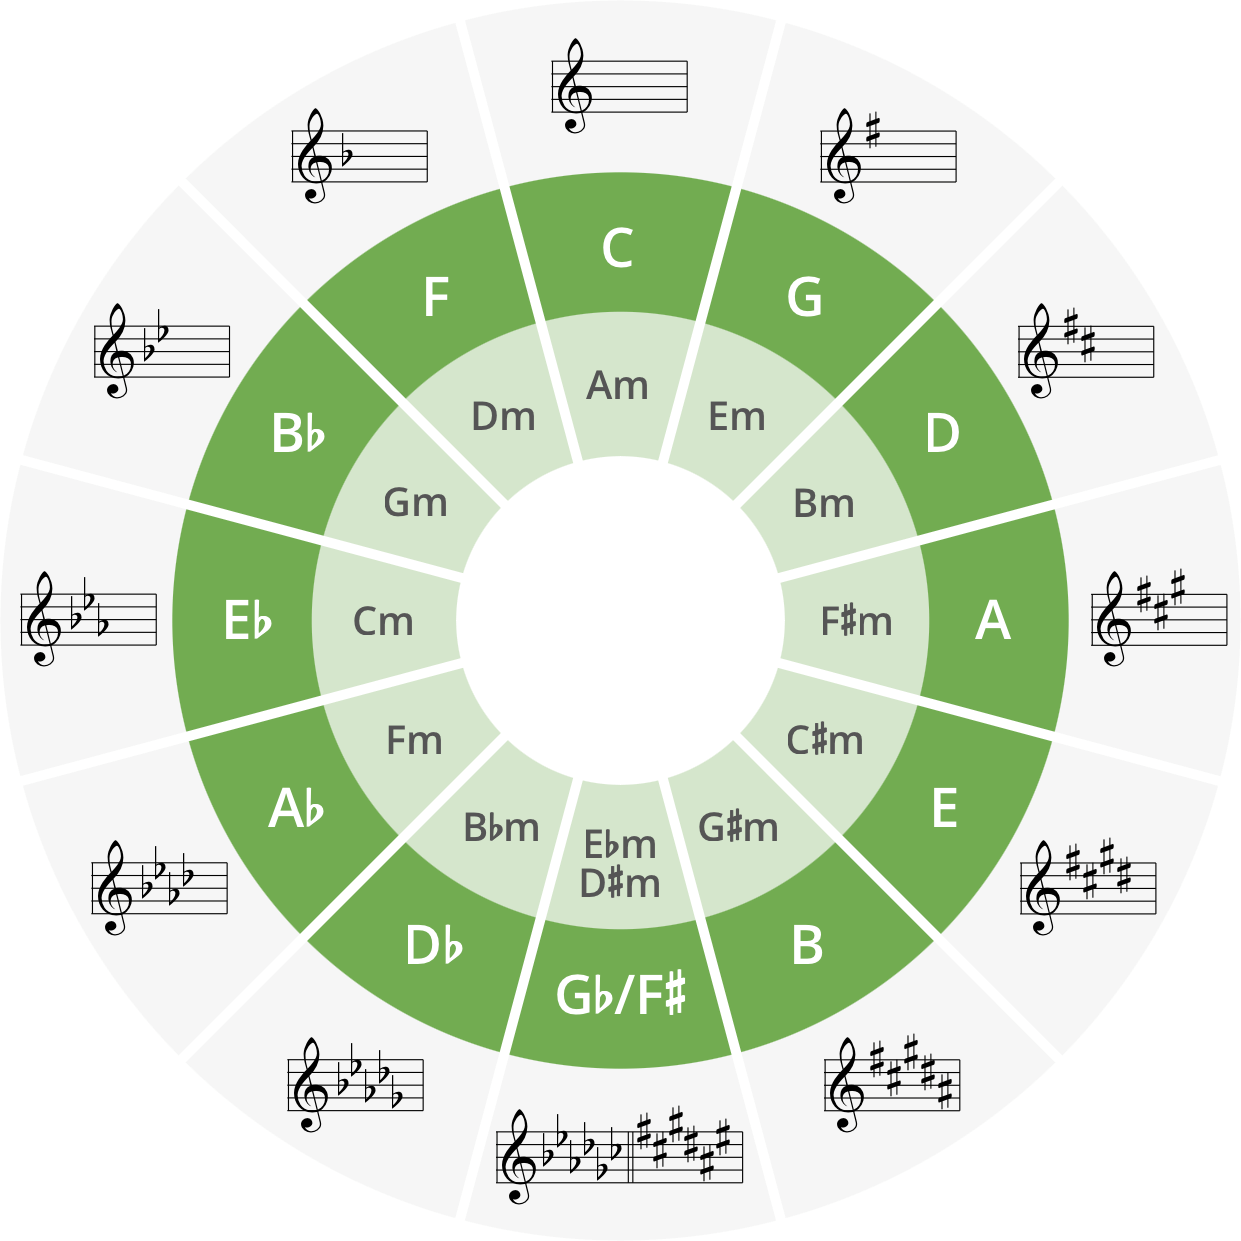
\includegraphics[width=.48\linewidth]{rys02/cof2.1}
	\caption{Wizualizacja koła kwintowego} \label{fig:kolokwintylowe}
\end{figure}

Koło kwintowe reprezentuje nuty ułożone na okręgu, przy czym nie są one ułożone według klasycznego zestawienia -- skali chromatycznej (C, C\#, D, D\#, E, F, F\#, G, G\#, A, A\#, B -- jedna gama dźwięków, odpowiadająca kolejnym klawiszom pianina), lecz za pomocą naturalnego ułożenia dźwięków. 
Przez naturalne ułożenie dźwięków należy rozumieć różnice pomiędzy częstotliwościami poszczególnych nut, na kole kwintowym są one ułożone w kolejności rosnącej, dzięki temu można w łatwy sposób dostrzec skąd biorą się poszczególne skale. Takie koło zostanie zaimplementowane jako jedna z funkcji autorskiej aplikacji.


Ważnym narzędziem dla muzyków jest metronom. Urządzenie to służy do wybijania rytmu, użytecznego przy okazji treningu słuchu oraz wyczuwania owego rytmu podczas gry. 
% DONE: w zaleceniach było, jak pisać agielskojęzyczne terminy !!!!!
Wymijanie rytmu można parametryzować. Określa się np.\ parametr bpm (ang.~\emph{beat per minute}) -- liczba uderzeń na minutę. Ponadto zwykle możliwe jest wybranie jednej z 4 opcji wyboru wybijania rytmu, bazujące na 4 podstawowych nutach. Są to: cała nuta -- jedno uderzenie na takt, pół nuta -- dwa uderzenia na takt, ćwierć nuta -- trzy uderzenia na takt, ósemka -- 4 uderzenia na takt. Działanie metronomu polega na wybijaniu poszczególnych taktów, podążając za ustalonym wcześniej tempem gry. 

Jeżeli chodzi o notację gitarową, to podczas realizacji niniejszej pracy posłużono się najbardziej rozpowszechnioną i czytelną formą. Do reprezentacji akordów (zbiorów nut, które grane ze sobą tworzą ujednolicony dźwięk) posłużono się widokiem gryfu gitarowego, przy czym czytając od góry reprezentowana jest kolejno 1, 2, 3, 4, 5, 6 struna gitary. Obok można dostrzec ich odpowiadające dźwięki, natomiast kropki symbolizują, które progi należy nacisnąć aby wydobyć oczekiwany dźwięk z instrumentu.

% DONE: przydałby się jakiś rysunek poglądowy - to jescze nie jest makieta, ale ilustracja do opisanych podstaw

\begin{figure}[htb]
	\centering
	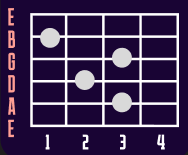
\includegraphics[width=.4\linewidth]{rys02/akord2.2}
	\caption{Wizualna reprezentacja akordu} \label{fig:pageLayout}
\end{figure}

W graficznej reprezentacji akordów pojawiają się określenia: major, minor, sus4, minor7, 7, 9, sus2, maj7, 7\#9, 5. Są to ustalone zbiory nut tworzące poszczególne akordy. Uwzględnienie wszystkich wariacji akordów jest istotne ze względów kompozycyjnych, gdyż poszerza horyzonty muzyków na tworzenie nowych dźwięków, nie ograniczając przy tym ich kreatywności. 

Istotnym aspektem w tworzeniu muzyki jest umiejętność rozpoznawania dźwięków posługując się tylko i wyłącznie słuchem. Posiadanie takiej umiejętności zwykło się nazywać ,,słuchem absolutnym'' dlatego też zawarto w aplikacji trening słuchu, odgrywający losową nutę, którą użytkownik następnie winien odgadnąć.  

\section{Przegląd dostępnych aplikacji}
Poniżej przedstawiono dwie wybrane aplikacje internetowe oferujące materiały oraz narzędzia do nauki gry na gitarze. 

\subsection{Guitar Tuna}
Jedną z większych i cieszących się dużą popularnością aplikacji jest \emph{Guitar Tuna}, oferowana w~ramach platformy \cite{Yousician}. Aplikacja ta jest przeznaczona w głównej mierze na urządzenia mobilne, z ograniczoną ilością funkcji na urządzenia desktopowe. Do oferowanych w niej narzędzi zalicza się: stroik i akordy  (patrz rysunek~\ref{fig:guitartuna}).
\begin{figure}[htb]
	\centering
	\begin{tabular}{ll}
	a) & b) \\
	\vtop{\vskip-2ex\hbox{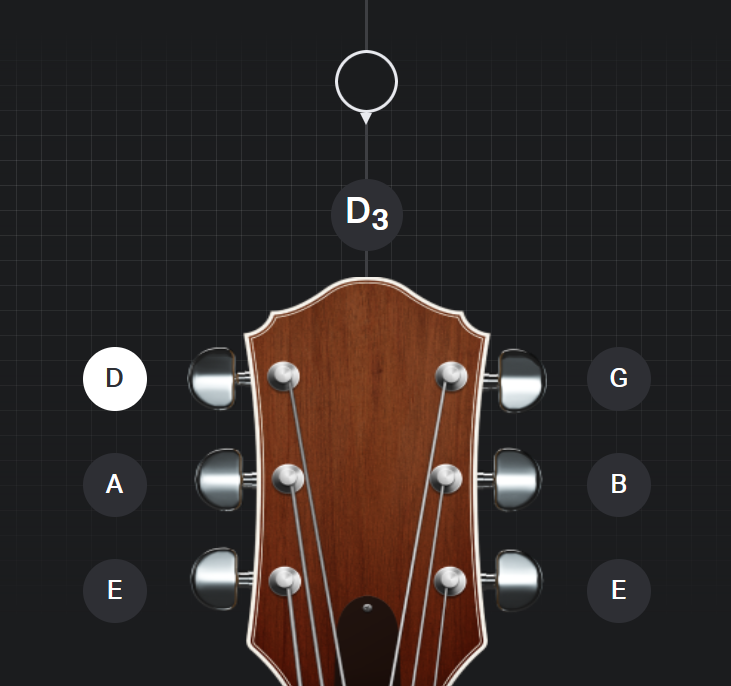
\includegraphics[width=.48\linewidth]{rys02/GTSTROIK}}} &
	\vtop{\vskip-2ex\hbox{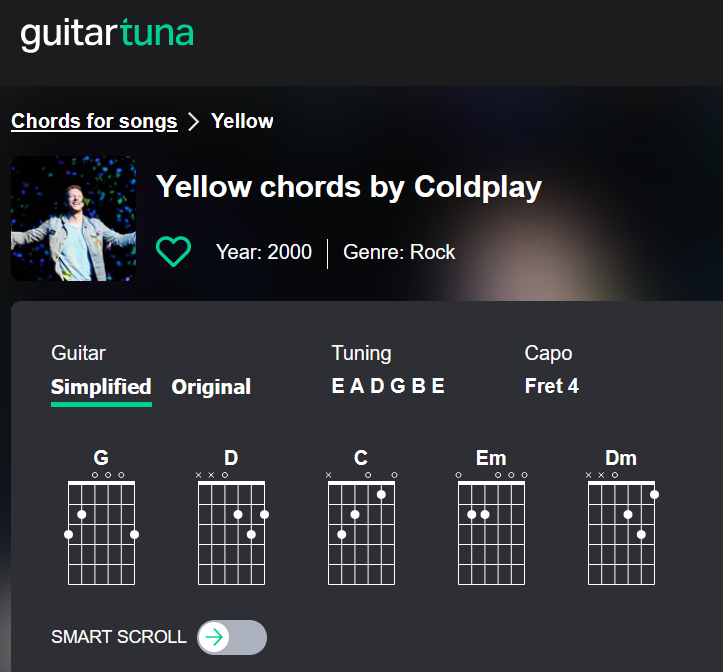
\includegraphics[width=.48\linewidth]{rys02/ChordsGT}}} 
	\end{tabular}
	\caption{Narzędzia dostępne w aplikacji Guitar Tuna: a) stroik, b) sekcja akordów aplikacji} \label{fig:guitartuna}
\end{figure}

\paragraph{Stroik} Stroik gitarowy pokazuje graficznie zagrany ton oraz ,,odległość'' od domniemanej nuty. Narzędzie umożliwia parametryzację polegającą na wyborze docelowej nuty do jakiej chcemy dostroić instrument. Narzędzie umożliwia też wybór instrumentu, wraz z jego graficzną reprezentacją na ekranie i przypisanymi nazwami nut obok odpowiadających pokręteł. Użytkownik do wyboru ma takie instrumenty jak gitara, ukulele, gitara basowa. Dodatkowym atutem jest możliwość wyboru niestandardowych strojeń instrumentów. 

\paragraph{Akordy} Sekcja akordów witryny internetowej jest uboższa aniżeli w aplikacji mobilnej. Narzędzie to daje dostęp do licznych piosenek, przy których przedstawione zostały akordy potrzebne do ich zagrania, wraz z tekstem i przejściami akordów w odpowiednich momentach. Zostało to zrobione statycznie, bez informacji na temat tempa utworu, czy dynamiki przejść pomiędzy granymi akordami. Istnieje tu również myląca funkcja "smart scroll" sugerująca możliwość grania wraz z podkładem grającym w tle, po naciśnięciu przycisku pojawia się jedynie odnośnik do pobrania aplikacji mobilnej.\\


Podsumowując powyższe obserwacje można stwierdzić, że aplikacja sama w sobie jest bardzo przystępna i intuicyjna, największym atutem jest stroik dający dowolność jeżeli chodzi o~używany instrument. Wersja desktopowa jest jednak znacznie okrojona w porównaniu do aplikacji mobilnej, nie znajdziemy tu listy akordów, diagramów skal czy metronomu. 

\subsection{TrueFire}
Aplikacja ta oferuje w większości płatne lekcje i materiały edukacyjne do gry na gitarze:

\begin{itemize}
    \item podkłady muzyczne do gry,
    \item kursy nauki gry poszczególnych stylów muzycznych np. blues, funk czy jazz,
    \item możliwość wykupienia prywatnych lekcji u instruktorów,
    \item transkrypcje znanych piosenek z instrukcjami gry,
\end{itemize}

Poza tym sama witryna zawiera sekcję z narzędziami do nauki (patrz rysunek~\ref{fig:truefire}). Właśnie te narzędzia poddano analizie pod względem użyteczności, czytelności, sposobu przedstawienia poszczególnych elementów.
\begin{figure}[htb]
	\centering
	\begin{tabular}{ll}
	a) & b) \\
	\vtop{\vskip-2ex\hbox{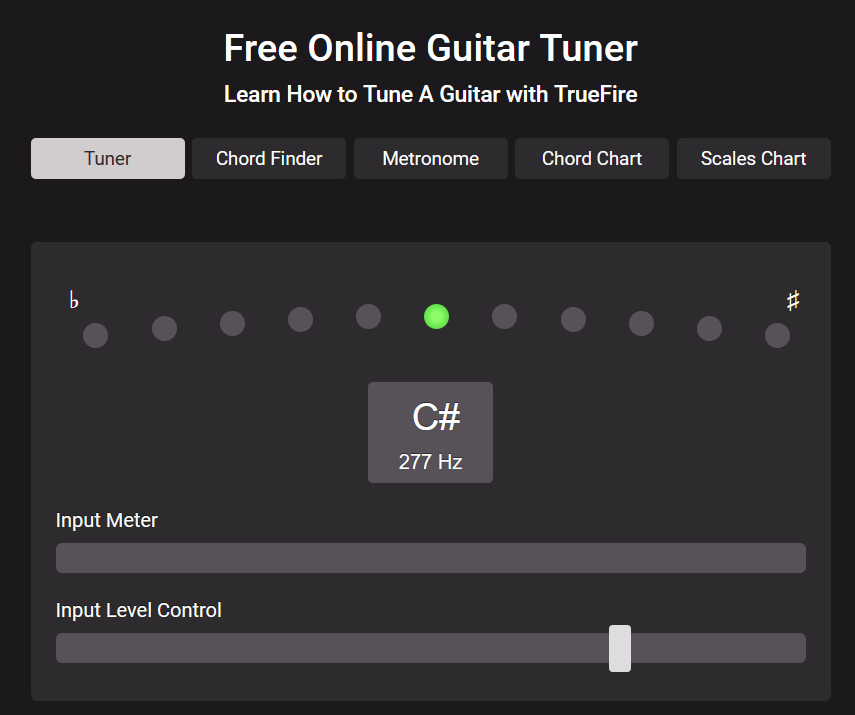
\includegraphics[width=.48\linewidth]{rys02/tuneFireStroik}}} &
	\vtop{\vskip-2ex\hbox{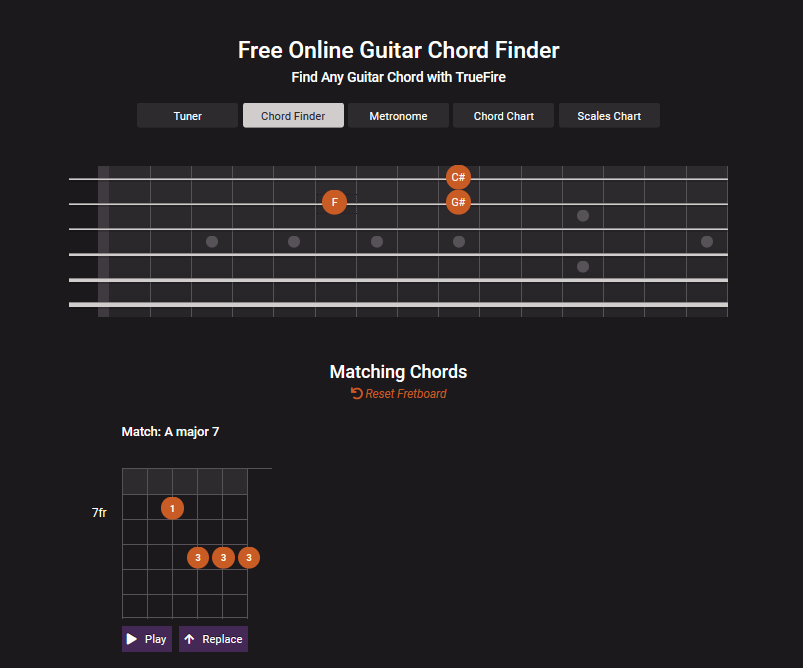
\includegraphics[width=.48\linewidth]{rys02/ChordFinder}}} \\
	c) & d) \\
	\vtop{\vskip-2ex\hbox{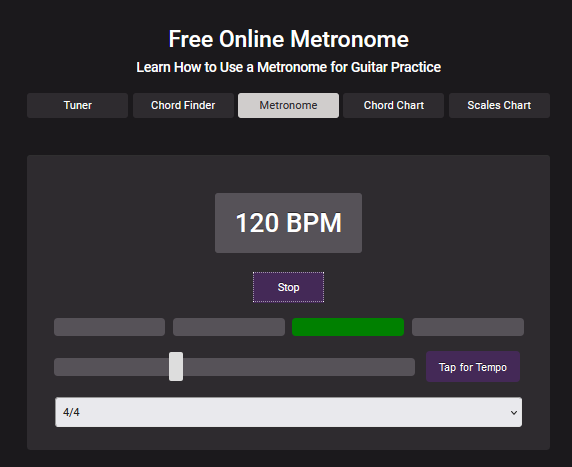
\includegraphics[width=.48\linewidth]{rys02/METRO}}}&
	\multirow{3}{*}{\vtop{\vskip-2ex\hbox{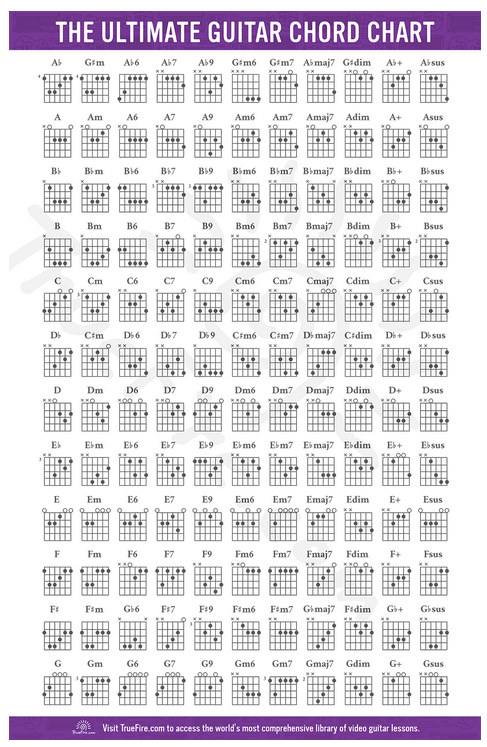
\includegraphics[width=.48\linewidth]{rys02/ChordChart}}}}	\\
	e) & \\
	\vtop{\vskip-2ex\hbox{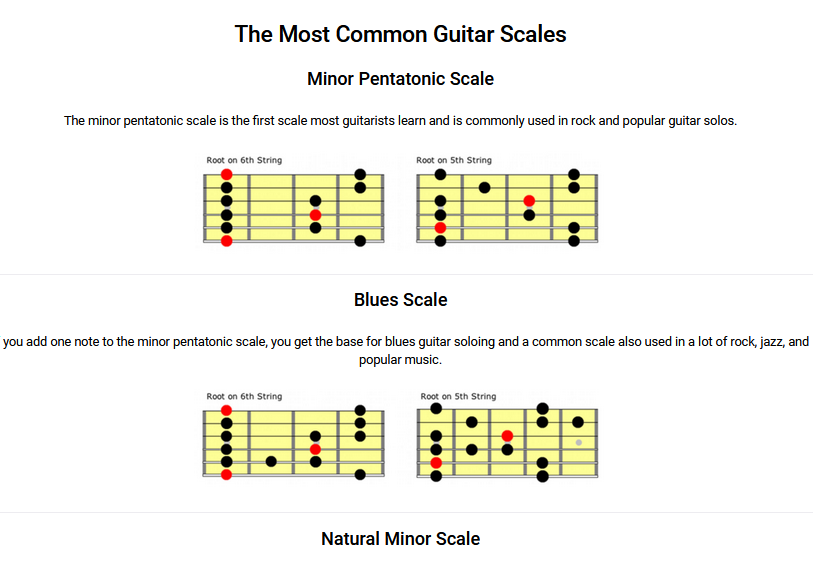
\includegraphics[width=.48\linewidth]{rys02/SKALETF}}} & 
	\end{tabular}
	\caption{Narzędzia dostępne w aplikacji TrueFire: a) stroik, b) eksplorator akordów, c) metronom, d) księga akordów, e) diagram skal} \label{fig:truefire} % TO DO: etykiety nie mogą się powtarzać !!!!!
\end{figure}

\paragraph{Stroik}
Został skonstruowany w sposób bardzo prosty -- rozpoznaje poszczególne dźwięki skali chromatycznej. Zawiera on w sobie \emph{input meter}, będący indykatorem poziomu decybeli dostarczanych do mikrofonu. Ma on również \emph{slider} umożliwiający parametryzację czułości mikrofonu. Samo narzędzie naturalnie umożliwia dostrojenie gitary do poszczególnych dźwięków, może być ono natomiast mało intuicyjne dla początkujących graczy, którzy nie są zapoznani z~domyślnym strojeniem strun gitary.

\paragraph{Eksplorator akordów}
Na podstawie zaznaczonych pozycji naciśniętych progów narzędzie to przeszukuje dostępne akordy, wyświetlając najbardziej podobne do zaznaczonych pozycji. Samo narzędzie jest z całą pewnością bardzo kreatywne. Jednak do samej nauki gry wydaje się być mało przydatne. Brak w nim kontekstu przy wyświetlanych znalezionych akordach oraz informacji odnośnie skal, do których sam akord należy. Algorytm dopasowujący nawet w przypadku podania losowych pozycji naciśniętych progów wygeneruje prawidłowe akordy. Może to być mylące dla nowych graczy, którzy błędnie mogą uznać podany przez nich układ jako wpisujący się pod prawidłowe akordy uznawane przez teorię muzyki.

\paragraph{Metronom}
Zaimplementowany jest w sposób prosty, dostarczając wszystkie potrzebne funkcje w jasny i przejrzysty sposób. Dla użytkownika dostępne są funkcje zmiany tempa wybijania poszczególnych bić, możliwość ręcznego ustawienia tempa, oraz dobór metrum z listy 6 dostępnych. Sama realizacja tej funkcji mogłaby zawierać dodatkowo opcję wyboru całych nut, a nie jedynie pół nut i ósemek przy wyborze metrum. Poza tym narzędzie spełnia swoje zadanie.

\paragraph{Księga akordów}

Zaprezentowana została w mało przystępny sposób. Mianowicie w aplikacji prezentowany jest diagram w formie statycznego obrazka, z mało czytelnym podziałem pomiędzy poszczególnymi akordami. Diagram ten jest wadliwy z powodu jego nieczytelności. Z powodu braku kontekstu pod akordami może też być niezrozumiały dla graczy początkujących, jak i średnio zaawansowanych. Same diagramy nie obrazują numeru progu, na którym dany akord ma być grany oraz nie przedstawia nuty odpowiadającej danej strunie.

\paragraph{Diagramy skal}
Przedstawiają one 6 najpopularniejszych skal muzycznych. Brakuje jednak możliwości przeniesienia tych diagramów poprzez gryf, wraz z informacją na temat tego w jakiej skali grany miałby być poszczególny diagram. Jest to rozwiązanie wadliwe, nie dostarczające wystarczająco dużej ilości informacji. \\


Podsumowując powyższe można uznać, że narzędzie dostarcza podstawowych funkcji umożliwiających naukę gry na gitarze, trening rytmu oraz możliwość dostrojenia samego instrumentu. Same funkcje natomiast zostawiają dużo miejsca na rozwój, np.\ przez parametryzację czy też umieszczenie informacji kontekstowych, objaśnienie pewnych sformułowań związanych z pozycjami akordów na gryfie. Narzędzie wyszukiwania akordów na podstawie podanych numerów progów może być mylące. Najbardziej przydatnym narzędziem z zestawienia jest metronom. 

\section{Wnioski}
% DONE: proszę nawiązać trochę do teorii z początku rozdziału
%        potem można przejść do oceny końcowej aplikacji
%        Chodzi o to, by rozdział był spójny - wnioski mają być podsumowaniem całego rozdziału

Przyglądając się wymienionym aplikacjom można dostrzec brak implementacji funkcji koła kwintowego w obydwu rozwiązaniach, będącym ważnym elementem jeżeli chodzi o początki nauki teorii muzyki. Użytkownik podczas korzystania z aplikacji nie ma możliwości zapoznania się z terminami skal muzycznych. Funkcja metronomu pomimo możliwości parametryzacji tempa nie gwarantuje możliwości wyboru wszystkich dostępnych nut wymienionych w pierwszej części rozdziału. Istniejące natomiast narzędzie diagramów skal nie dostarcza wystarczającej ilości informacji, aby uznać je za narzędzie skończone. Biorąc pod uwagę notację gitarową można dostrzec brak ujednoliconego sposobu reprezentacji akordów, wykorzystywane są dwie różne wariacje, przy których również nie znajdziemy pomocy kontekstowej. Do dobrych cech aplikacji można zaliczyć prostotę ich obsługi, zwłaszcza w narzędziu stroika aplikacji Guitar Tuna oraz metronomu Truefire. Do największych wad należy brak kontekstu przy wizualizacji listy dostępnych akordów, oraz ograniczoną ilość możliwości przy wersji desktopowej aplikacji.



\chapter{Założenia projektowe}
% DONE?: Zamieszczono analizę wymagań, funkcjonalnych i niefunkcjonalnych, razem z wizualizacją funkcji za pomocą makiet \\\  zwykle projekty informatyczne zaczynają się od studium wykonalności (i analizy dziedzinowej).
%        Potem pojawia się analiza wymagań, której wynikiem jest zestaw zachowań, jakimi powinna
%        charakteryzować się powstająca aplikacja z punktu widzenia użytkownika.
%        W efekcie po tym etapie powinno być wiadome, jakie aplikacja będzie oferować funkcje i do czego ma służyć.
%       U Pana etap analizy wymagań nie został wyraźnie zaznaczony. 
%       Analizę wymagań formalizuje się, stosując listy wyliczeniowe, diagramy przypadków użycia itp.
%       Temu wszystkiemu towarzyszyć mogą makiety interfejsu użytkownika.
%       Makiety służą bowiem jako język, którym projektant komunikuje się z użytkownikiem.
%       Są one też językiem komunikacji między projektantem a programistą
%       Ogólnie - tworzenie makiet można zaliczyć do etapu analizy wymagań funkcjonalnych
%       (makiety eksponują funkcje, które są wystawiane na graficznym interfejsie użytkownika)
W niniejszym rozdziale opisano szczegóły działań, jakie podjęto po analizie dziedzinowej. W~ich ramach zdefiniowano wymagania funkcjonalnych i niefunkcjonalnych dla budowanej aplikacji. Na tej bazie przystąpiono do zaprojektowania makiet interfejsu użytkownika. Następnie zdecydowano się na wybór wzorca projektowego, na podstawie którego miała się odbywać implementacja komponentów wchodzących w skład poszczególnych scen. Po zadeklarowaniu potrzebnych elementów przystąpiono do tworzenia grafik tych komponentów, w tym: grafiki przycisków, tekstu, grafik akordów. Następnie zajęto się implementacją widoków i funkcji. 

\section{Analiza wymagań}
\subsection{Wymagania funkcjonalne}
Docelowa aplikacja powinna oferować funkcje opisane poniżej.
\begin{itemize}
\item \textbf{Stroik gitarowy} -- ta funkcja powinna umożliwiać dostrojenie strun gitary. Zawierać on ma opcję wyboru nuty, do której struna ma docelowo zostać nastrojona. Stroik zawierać ma graficzną reprezentację aktualnego poziomu nastrojenia instrumentu, poprzez wyświetlanie na ekranie informacji, czy struna jest: niedostrojona, nastrojona, przestrojona.
\item \textbf{Metronom} -- ma umożliwiać przeprowadzenie treningu rytmu, pozwalająć na parametryzację wartości: bpm, taktu.
\item \textbf{Księga akordów} -- ma dostarczać informacje o aktualnie wyświetlanym akordzie i jego wariacji. Zawierać ona ma również przycisk zezwalający na zapis aktualnie wyświetlanego akordu, z możliwością zapisu do 3 akordów, które następnie dostępne będą w osobnym widoku. Osobny widok zawierać ma również diagram akordów.
\item \textbf{Koło kwintowe} -- ma się pojawiać z aktywnymi przyciskami, których naciśnięcie skutkować ma podświetleniem skali durowej, wraz z sześcioma akordami, które wpasowują się pod wybraną nutę.
\item \textbf{Trening słuchu} -- istotą tej funkcji ma być możliwość odgadywania odegranej nuty poprzez jej zagranie i zweryfikowanie poprawności udzielonej odpowiedzi. 
\end{itemize}

\subsection{Wymagania niefunkcjonalne}

Dla projektu ustalono wymagania niefunkcjonalne. Zebrano je w punktach poniżej.
\begin{itemize}
\item \textbf{Intuicyjny interfejs} -- aplikacja ma oferować prosty i przejrzysty interfejs, z możliwością włączenia pomocy kontekstowej wyjaśniająca działanie poszczególnych elementów w widoku.
\item \textbf{Kompatybilność z systemem Windows 10} --  aplikacja zostanie stworzona głównie dla urządzeń desktopowych, działających pod kontrolą systemu operacyjnego Windows 10 (i wyżej).
\item \textbf{Responsywność} -- czas odpowiedzi aplikacji nie powinien wynosić więcej niż 2 sekundy. 
\end{itemize}
% DONE?: Wyjaśnienie zamieszczone w podrozdziale "przebieg" \\\ proszę dodać wyjaśnienie, jaką ścieżką Pan poszedł rozpoczynając projekt.
%        z tego, co widzę, całą analizę wymagań załatwił Pan makietami. 
%        W sumie można tak zrobić. Proszę to jednak uzasadnić, by czytelnik nie miał wątpliwości, 
%        że to celowy zabieg, a nie przeoczenie !!! 


% DONE?: proszę przeredagować rozdział. W tej chwili wygląda on słabo - nie widać jakiejś myśli przewodniej.

% DONE: proszę uważać ze stosowaniem określenia "architektura aplikacji"
%        zwykle gdy pada to określenie to odnosi się ono do sposobu "poukładania" komponentów aplikacji w jakieś hierarchie czy warstwy, z wydzieleniem odpowiedzialności, określeniem mechanizmów przepływu informacji itd. U Pana zaś mamy termin ten pada w kontekście użycia wzorca projektowego MVC.

\section{Makiety}
Na rysunku~\ref{fig:makiety} przedstawiono zaprojektowane makiety interfejsu użytkownika. Makiety te mają przybliżyć ogólny zarys planowanego układu udostępnianych widoków wraz z rozmieszczeniem na nich funkcji. Końcowa wersja interfejsu użytkownika może odbiegać od tej propozycji.
\begin{figure}[htb]
    \centering
		\begin{tabular}{ll}
		a) & b) \\
		\vtop{\vskip-2ex\hbox{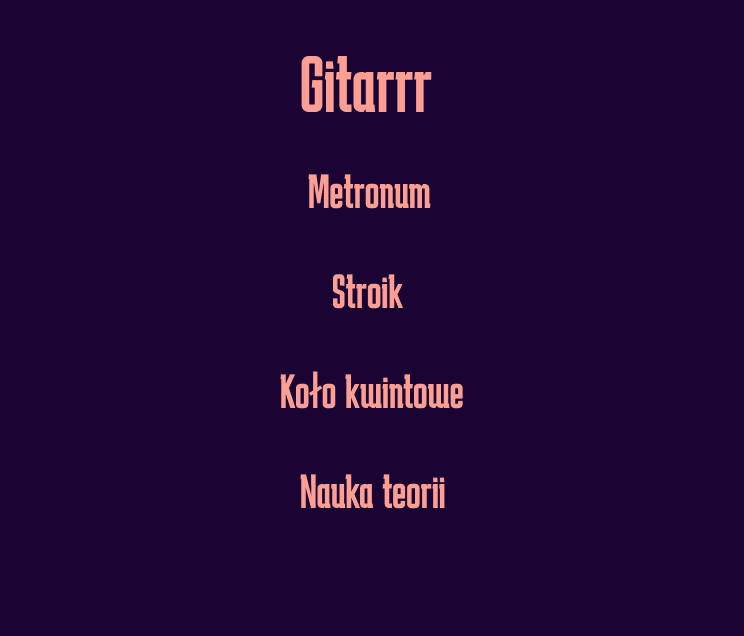
\includegraphics[width=0.4\linewidth]{rys03/MakMain}}} &
		\vtop{\vskip-2ex\hbox{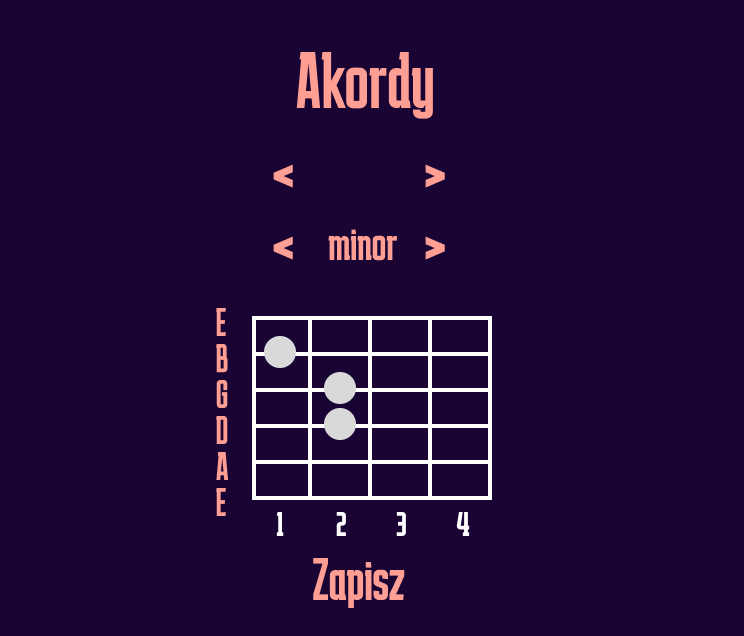
\includegraphics[width=0.4\linewidth]{rys03/MakAkordy}}} \\
		c) & d) \\
		\vtop{\vskip-2ex\hbox{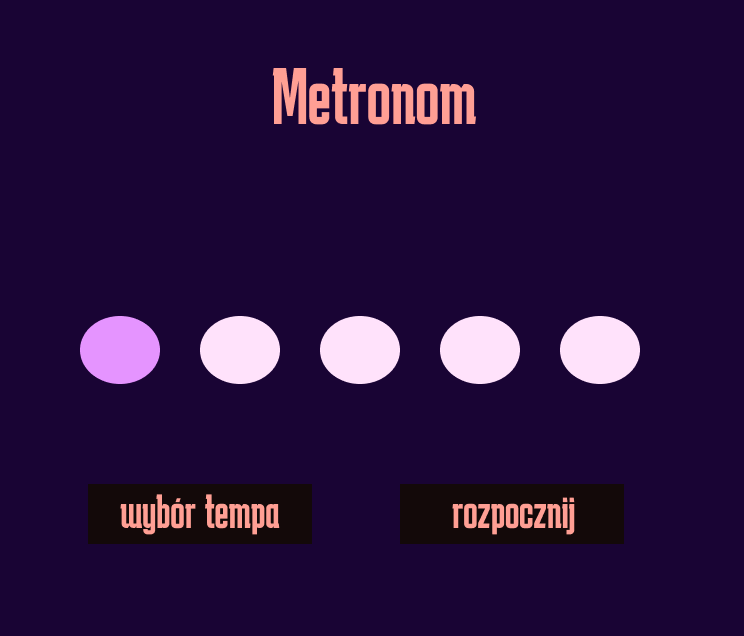
\includegraphics[width=0.4\linewidth]{rys03/MakMetronom}}} &
		\vtop{\vskip-2ex\hbox{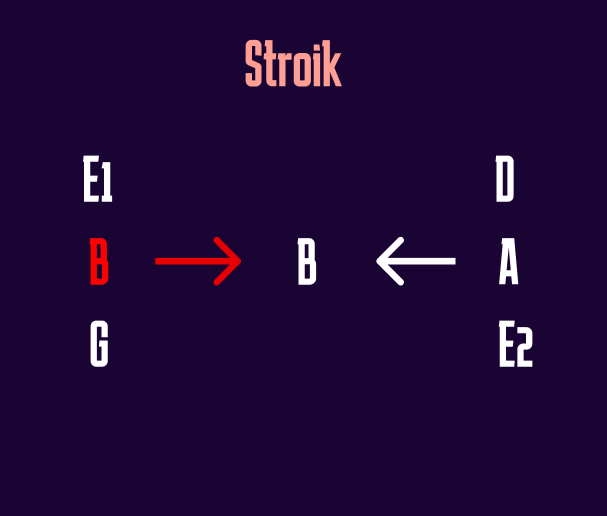
\includegraphics[width=0.4\linewidth]{rys03/MakStroik}}} \\
		e) & f) \\
		\vtop{\vskip-2ex\hbox{
\includegraphics[width=0.4\linewidth]{rys03/MakTrening}}} &
		\vtop{\vskip-2ex\hbox{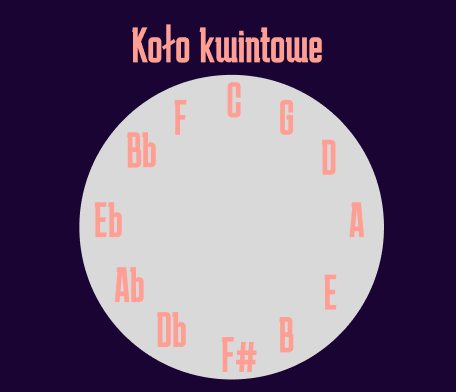
\includegraphics[width=0.4\linewidth]{rys03/MakKK}}}	
		\end{tabular}
        \caption{Zaprojektowane makiety interfejsu: a) scena główna, b) księga akordów, c) metronom, d) stroik, e) trening słuchu, f) koło kwintowe}
        \label{fig:makiety}
\end{figure}


\section{Projekt aplikacji}
% DONE: proszę zadbać o to, by na końcach linii nie pozostały samotne literki
Projekt aplikacji stworzono w sposób taki, aby każda z poszczególnych funkcji była przejrzysta, a sama aplikacja umożliwiała płynne przełączanie pomiędzy widokami. Zastosowano wzorzec \emph{Model-View-ViewModel}, umożliwiający rozdzielenie logiki aplikacji, interfejsu oraz zarządzania danymi. W skład wzorca wchodzą poniższe 3 elementy:

\begin{itemize}
	\item \emph{Model}: Logika danych aplikacji, zawierająca dane akordów, dźwięków, tempo metronomu,
	\item \emph{View}: Zawiera sceny samej aplikacji, dla każdej funkcji zaplanowano osobny widok (sceny),
	\item \emph{ViewModel}: Do każdej ze scen przypisany został kontroler odpowiedniej sceny umożliwiający komunikację pomiędzy widokiem, a modelem, zawiera on logikę aplikacji, oraz definicje funkcji potrzebnych w danej scenie.
\end{itemize}

\subsection{Projekt poszczególnych scen}
Poniżej omówiono schemat każdej z projektowanych scen aplikacji, zaznaczając komponenty wchodzące w skład danego narzędzia, wyjaśniając co jest ich celem oraz jakie technologie wykorzystano w ich implementacji. 

\subsubsection{Scena 1: Scena Główna}

\begin{itemize}

\item Cel: Reprezentacja możliwości wyboru, oraz udzielenie użytkownikowi dostępu do poszczególnych narzędzi za pomocą czytelnych przycisków, które po naciśnięciu przechodzą do odpowiadającej im sceny z danym narzędziem. 
\item Komponenty: Elementami wchodzącymi w skład sceny głównej są przyciski (jest ich 5): stroik, metronom, koło kwintowe, księga akordów, trening słuchu. Dodatkowo scena główna zawiera obiekt tekstowy z logiem i przycisk odpowiedzialny za zamknięcie aplikacji.  
\item Technologie: Do realizacji tej oto sceny użyto wbudowaną bibliotekę w silnik Unity, a mianowicie Unity.UI \cite{UnityUI}, umożliwiającą utworzenie graficznego interfejsu uzytkownika. 
\item Komunikacja: Każdy z przycisków wchodzących w skład sceny podłączony jest pod kontroler sceny, służący jako pośrednik, w skrypcie należącym do kontrolera poszczególnym przyciskom przypisywana jest funkcja odpowiadająca za załadowanie odpowiedniej sceny. 
\end{itemize}

\subsubsection{Scena 2: Stroik}

\begin{itemize}
\item Cel: Udostępnienie możliwości nastrojenia gitary poprzez wybór docelowej struny, do której użytkownik chce nastroić instrument. Następnie zagrane przez użytkownika dźwięki analizowane będą, a wyniki analizy reprezentowane zostaną jako informacja odnośnie tego, czy ton należy obniżyć czy podwyższyć.
\item Komponenty: W skład sceny wchodzi mikrofon, analizator dźwięku, przyciski odpowiadające strunom na gitarze, oraz indykator aktualnego poziomu nastrojenia instrumentu.  
\item Technologie: Do użytych technologii wykorzystano bibliotekę opartą na otwartej licencji służącą do analizy dostarczanego dźwięku \cite{AudioPitchEstimator}, oraz wyciągnięcie z niego częstotliwości zagranej nuty. Dodatkowo do stworzenia graficznego interfejsu posłużono się biblioteką Unity.UI. Użyto też komponentu audio wbudowanego w silnik Unity \cite{AudioSource}.
\item Komunikacja: Użyto kontroler sceny, aby umożliwić komunikacje pomiędzy elementami graficznymi a analizatorem dźwięku. 
\end{itemize}

\subsubsection{Scena 3: Metronom}

\begin{itemize}
\item Cel: Zapewnienie użytkownikowi możliwości treningu rytmu podczas gry, poprzez reprezentację poszczególnych taktów zsynchronizowanych z dźwiękiem ,,bitu''.
\item Komponenty: Do realizacji tej sceny zastosowano przyciski umożliwiające parametryzację taktu, oraz bpm(ang. beats per minute). Wizualizacja metronomu odbywa się za pośrednictwem pojawiających się na ekranie kwadratów reprezentujących poszczególny takt, które zmieniają swoje kolory z białego na czarny, wraz z czasem wybijania danego rytmu.
\item Technologie: Kod napisany w języku C\# realizujący logikę działania metronomu, komponent audio.
\item Komunikacja: Poszczególne komponenty komunikują się ze sobą za pośrednictwem kontrolera sceny metronomu, zawierający odwołania do poszczególnych komponentów.
\end{itemize}

\subsubsection{Scena 4: Księga akordów}

\begin{itemize}
\item Cel: Wizualizacja pozycji akordów na gryfie, dla każdej nut, wraz z możliwymi wariancjami akordów.
\item Komponenty: Do komponentów należą przyciski odpowiadające za przeglądanie listy dostępnych akordów, zapisu akordu, element graficzny wizualizujący aktualnie wybrany akord, wraz z przyciskami odpowiadającymi za przełączenie sceny do widoku diagramu wszystkich możliwych i zapisanych akordów.
\item Technologie: Wbudowana biblioteka do obsługi graficznego interfejsu użytkownika - Unity.UI.
\item Komunikacja: Komponenty komunikują się ze sobą za pomocą menadżera sceny, przechowującego za pomoca listy graficzne reprezentacje akordów, które wyświetlane są w odpowiednich momentach. 
\end{itemize}

\subsubsection{Scena 5: Trening słuchu}

\begin{itemize}
\item Cel: Umożliwienie użytkownikowi przeprowadzenie ćwiczeń mających na celu nabycia umiejętności rozpoznawania granej nuty za pomocą samego słuchu.
\item Komponenty: Przyciski odpowiadające za wybór skali treningowej, przyciski odpowiadające za odpowiedź, po naciśnięciu których weryfikowana jest poprawność udzielonej odpowiedzi. Scena zawiera również system audio odpowiadający za odegranie dźwięku. Zawiera też przycisk reset, oraz przycisk odpowiedzialny za odegranie dźwięku.
\item Technologie: Za odgrywanie dźwięków odpowiada biblioteka Unity, wraz z gotowym komponentem audio wbudowanym w silnik Unity.
\item Komunikacja: Za komunikację pomiędzy komponentami odpowiada menadzer sceny, łączący ze sobą przyciski, zawierający logike odpowiedzialną za działanie sceny.
\end{itemize}

\subsubsection{Scena 6: Koło kwintowe}

\begin{itemize}
	\item Cel: Wizualizacja koła kwintowego, wraz z skalą molową i durową.
	\item Komponenty: Elementy graficzne, w postaci przycisków, zawierające komponent \texttt{text}, który zawiera odpowiadającą nutę.
	\item Technologie: Użyto biblioteki Unity.UI do reprezentacji poszczególnych nut.
	\item Komunikacja: Komunikacja odbywa się poprzez menadżer sceny, zawierający logikę odpowiadającą za podświetlenie odpowiadających nut po naciśnięciu jednego z przycisków na kole kwintowym.
\end{itemize}

\subsubsection{Scena 7: Diagram akordów}

\begin{itemize}
	\item Cel: Wizualizacja wszystkich dostępnych akordów w aplikacji.
	\item Komponenty: Elementy graficzne, w postaci przycisków, zawierające komponent image, który zawiera odpowiadający akord.
	\item Technologie: Użyto biblioteki Unity.UI do reprezentacji poszczególnych nut.
	\item Komunikacja: Komunikacja odbywa się poprzez menadżer sceny, zawierający logikę odpowiadającą za uruchomienie widoku księgi akordów z wyświetlonym wybranym akordem.
\end{itemize}

\subsubsection{Scena 8: Zapisane akordy}

\begin{itemize}
	\item Cel: Wizualizacja zapisanych przez użytkownika akordów w scenie księgi akordów.
	\item Komponenty: Elementy graficzne zawierające komponent image, który zawiera odpowiadający akord.
	\item Technologie: Użyto biblioteki Unity.UI do reprezentacji poszczególnych akordów.
	\item Komunikacja: Komunikacja odbywa się poprzez menadżer sceny, zawierający logikę odpowiadającą komunikację ze sceną księgi akordów i przekazaniu zapisanych akordów.
\end{itemize}
\chapter{Implementacja}

\section{Wprowadzenie do implementacji}

%TODO wrzucić listingi

Rozdział ten zawiera szczegóły implementacji aplikacji. Każdej scen poświęcono odpowiadający podrozdział wyjaśniający wykorzystane technologie, biblioteki oraz sposób komunikacji pomiędzy poszczególnymi elementami widoku. 

% TO DO: w rozdziale dobrze byłoby zamieścić opis struktury projektu. Ponieważ rozwijał Pan aplikację w środowisku UNITY, to środowisko narzuca trochę tę strukturę (parę uwag na ten temat też by się przydało). Strukturę projektu można pokazać robiąc zrzuty drzewa źródeł kodu.

% TO DO: przydałoby się też opowiedzieć trochę o budowaniu aplikacji (testowe uruchomienia odbywają się w środowisku, aby można było uruchomić aplikację poza tym środowiskiem - coś trzeba przecież zrobić).


\section{Implementacja elementów aplikacji}

\subsection{Stroik}

Głównymi elementami sceny sa przyciski służące do wyboru domniemanej nuty. W skład widoku wchodzi tez jej tytuł, informator odnośnie aktualnego poziomu nastrojenia instrumentu i przyciski odpowiedzialne za zmianę docelowego instrumentu. Do menadżera sceny przypięte zostały 3 skrypty realizujące logikę potrzebną do nagrania, przeanalizowania i wyświetlenia wyników analizy dźwięku. Nazwy tych skryptów to: \texttt{Audio Recorder} - skrypt odbierający dźwięk ze sceny, \texttt{Audio Pitch Estimator} - odpowiedzialny za analizę odebranego dźwięku, \texttt{Tuner Manager} - główny skrypt realizujący logikę sceny. 

Skrypt \texttt{Audio Recorder} zawiera dwa pola:
\begin{itemize}
    \item \texttt{audioSource} -- obiekt przechowujące odwołanie do wbudowanego w silnik Unity narzędzia \texttt{AudioSource}, umożliwiającego nagranie dźwięku,
    \item \texttt{duration} -- zmienna odpowiedzialna za ustalenie czasu, przez jaki mikrofon ma odbierać dźwięk z otoczenia.
\end{itemize}

Skrypt zawiera jedną funkcję \texttt{OnEnable}, która podczas uruchomienia zaczyna odbierać dźwięk dostarczany do mikrofonu. Skrypt \texttt{AudioPitchEstimator}, zaczerpnięty z repozytorium \cite{https://github.com/nakakq/AudioPitchEstimatorForUnity}, % TO DO: to nie jest poprawne cytowanie, proszę zrobić odpowiedni rekord w bib, a potem użyć jego klucza w \cite
służy do analizy odebranego dźwięku. Biblioteka zawiera poniżej wymienione zmienne, na które użytkownik może wpłynąć, aby dopasować narzędzie do swoich potrzeb.
\begin{itemize}
    \item \texttt{frequencyMin} -- minimalna częstotliwość, jaka ma być analizowana,
    \item \texttt{frequencyMax} -- maksymalna częstotliwość poddawana analizie,
    \item \texttt{harmonicsToUse} -- ilość harmonicznych jakie mają być brane pod uwagę, podczas ustalania końcowej częstotliwości odebranego dźwięku,
    \item \texttt{smoothingWidth} -- pasmo częstotliwości filtra wygładzającego widmo,
    \item \texttt{thresholdSRH} -- wartość graniczna decybeli, od której dźwięk ma być wzięty pod analizę.
\end{itemize}

Funkcją realizującą główną logikę działania jest metoda \texttt{Estimate}, wykonująca szybką transformatę Fouriera na odebranym dźwięku. Funkcja ta zwraca zmienną float \texttt{bestFreq}, będąca najlepszym możliwym według programu ,,trafieniem'', jeżeli chodzi o odebraną częstotliwość. Skrypt \texttt{TunerManager} odpowiedzialny za realizowanie logiki sceny, przechowuje odwołania do komponentów sceny: przyciski, pola tekstowe, obiekt \texttt{AudioSource}. W jego skład wchodzi 6 funkcji o nazwie \texttt{SetDesiredFrequency*}, przy czym każdemu z przycisków przypisany jest jeden jej odpowiednik, ustawiający parametry skryptu \texttt{AudioPitchEstimator}. Funkcją odpowiedzialną za logikę analizy dźwięku jest \texttt{EstimatePitch}, która korzysta ze skryptu \texttt{AudioPitchEstimator}, na tej podstawia ustawia wartości elementów tekstowych informujących użytkownika o poziomie nastrojenia instrumentu. Poza tym istnieją tu jeszcze dwie metody:

\begin{itemize}
    \item \texttt{Start} -- funkcja przypisująca przyciskom im działania w wypadku naciśnięcia.
    \item \texttt{ClearColor} -- funkcja pomocnicza, odpowiedzialna za ,,czyszczenie'' elementów graficznych sceny.
\end{itemize}

\subsection{Metronom}
Scena metronomu zawiera 9 przycisków służących do parametryzacji działania metronomu, umożliwiając zwiększenie tempa, zmianę metrum, zwiększanie lub zmniejszanie liczby taktów. Za logikę odpowiada menadżer sceny z przypiętym skryptem \texttt{MetronomeManager}, zawierający 10 pól obiektów przycisków, pole obiektu tekstowego i kilka zmiennych pomocniczych. Metronom realizowany jest za pomocą wizualizacji poszczególnych taktów za pomocą graficznych elementów w postaci "kółek", które dodawane sa do widoku dynamicznie w zależności od ustalonych przez użytkownika wartości. Funkcje jakie implementuje dany skrypt to:

\begin{itemize}
    \item \texttt{Start} -- funkcja odpowiadająca za ustawienie zmiennych, obiektów widoku. 
    \item \texttt{AddCircle} -- funkcja wykorzystywana do zwiększenia tempa.
    \item \texttt{DeleteCircle} -- funkcja wykorzystywana do zmniejszenia tempa.
    \item \texttt{RearrangeElements} -- funkcja stworzona do rozmieszczania ,,kółek'' taktów na ekranie.
    \item \texttt{StartMetronome} -- funkcja uaktywniająca metronom.
    \item \texttt{RecolorAll} -- funkcja uruchamiana podczas resetu metronomu, czyszcząca grafiki wizualizacji metronomu.
    \item \texttt{MetronomeCoroutine} -- oobny wątek odpowiedzialny za działanie metronomu, w czasie działania tej funkcji wybijane jest na ekranie tempo.
    \item \texttt{AddBpm} -- funkcja odpowiedzialna za zwiększenie tempa.
    \item \texttt{SubtractBpm} -- funkcja odpowiedzialna za zmniejszenie tempa.
    \item \texttt{ChangeMeasure*} -- funkcje, przypisane do odpowiednich przycisków, w zależności od wyboru całej nuty, pół nuty, ćwierć nuty czy ósemki, odpowiednio ustawiają ilość bić na takt.
\end{itemize}
\subsection{Księga akordów}

Scena księgi akordów zawiera element graficzny reprezentujący aktualnie wybrany akord gitarowy, przyciski umożliwiające wybór docelowego akordu, elementy graficzne ułatwiające nawigację po widoku sceny. Funkcje wchodzące w skład skryptu menadżera sceny nazwanego \texttt{ChordChartsManager} to:

\begin{itemize}
    \item \texttt{Start} -- funkcja odpowiedzialna za przygotowanie potrzebnych elementów sceny. Przypisuje grafiki akordów z pomocniczej listy Chords do listy głównej ch. Ustawia wartości zmiennych noteIterator, variantIterator z wartości przechowywanych w skrypcie SceneConnector, łączącej scenę księgi akordów z widokiem wszystkich akordów w postaci diagramu. Przypisuje ona funkcje do odpowiednich przycisków i resetuje wartości obiektów tekstowych.
    \item \texttt{noteIncrement} -- funkcja przypisana do przycisku, odpowiedzialna za zmianę nuty akordu.
    \item \texttt{noteDecrement} -- funkcja przypisana do przycisku, odpowiedzialna za zmianę nuty akordu.
    \item \texttt{variantIncrement} -- funkcja przypisana do przycisku, odpowiedzialna za zmianę wariacji akordu.
    \item \texttt{variantDecrement} -- funkcja przypisana do przycisku, odpowiedzialna za zmianę wariacji akordu.
    \item \texttt{ChangeVariantText} -- funkcja odpowiedzialna za zmianę przypisanej wartości obiektu tekstowego sceny, wykorzystywana w momencie zmiany wariacji akordu.
    \item \texttt{ChangeNoteText} -- funkcja odpowiedzialna za zmianę przypisanej wartości obiektu tekstowego sceny, wykorzystywana w momencie zmiany nuty akordu.
    \item \texttt{ChangeChord} -- funkcja odpowiedzialna za zmianę aktualnie wyświetlanego akordu, zmienia przypisaną grafikę obiektu Image sceny.
\end{itemize}

\subsection{Trening słuchu}

Scena treningu słuchu zawiera przycisk odpowiedzialny za odegranie dźwięku, który następnie ma zostać odgadnięty przez użytkownika za pomocą jednego z 12 przycisków obecnych na scenie. W skład sceny wchodzą dwa skrypty: \texttt{EarTrainerManager} -- przypisany do menadżera sceny realizujący główną logikę sceny oraz \texttt{ButtonIndex} -- skrypt pomocniczy przypisany do każdego z 12 przycisków odpowiedzialnych za udzielenie odpowiedzi. Funkcje wchodzące w skład głównego skryptu to:
\begin{itemize}
    \item \texttt{Start} -- funkcja przypisująca obiekt \texttt{audioSource}, odpowiedzialny za odgrywanie dźwięków. Ustawia ona również funkcję \texttt{PlayRandomNote} do przycisku \texttt{playNoteButton}. Dodatkowo przypisuje ona funkcję \texttt{NoteGuessed} do każdego z przycisków odpowiedzialnych za odpowiedź.
    \item \texttt{PlayRandomNote} -- funkcja odpowiedzialna za odegranie losowego dźwięku po naciśnięciu przycisku \texttt{playNoteButton}. Ustawia ona odpowiedni index dla odegranej nuty, wykorzystywany następnie podczas zweryfikowania odpowiedzi podanej przez użytkownika.
    \item \texttt{NoteGuessed} -- funkcja weryfikująca odpowiedź użytkownika, wykorzystywana po naciśnięciu jednego z 12 przycisków odpowiedzi. Ustawia ona obiekty tekstowe sceny, w zależności od tego czy odpowiedź była poprawna, czy też nie. 
\end{itemize}

Skrypt pomocniczy przechowuje jedynie jedną zmienną, wykorzystywaną w momencie weryfikacji odpowiedzi udzielonej przez użytkownika, jest nią: \texttt{buttonNumber}.

\subsection{Koło kwintowe}

Scena koła kwintowego zawiera 24 przyciski, każdemu z nich przypisana została odpowiednia nuta. W skrypcie menadżera sceny utworzone zostały dwie listy, przechowujące przyciski koła zewnętrznego oraz koła wewnętrznego. Skrypt zawiera w sobie 6 funkcji:

\begin{itemize}
\item \texttt{Start} -- funkcja używana podczas tworzenia obiektu, służy ona przygotowaniu wszystkich przycisków oraz przypisania im działania przy ich naciśnięciu, w tym przypadku przypisuje ich działanie do funkcji \texttt{DisplayScale}
\item \texttt{DisplayScale} -- funkcja odpowiedzialna jest ona za wyświetlenie skali majorowej, oraz 3 akordów minorowych pasujących do wybranej przez użytkownika nuty. 
\item \texttt{GetColorTin}t -- funkcja pomocnicza generująca kolejne odcienie kolorów, dla funkcji \texttt{DisplayScale}.
\item \texttt{GetMajorScaleIndices} -- funkcja pomocnicza generująca interwały kolejnych nut w skali majorowej.
\item \texttt{ChangeButtonColor} -- funkcja pomocnicza odpowiedzialna za zmianę koloru odpowiedniego przycisku.
\item \texttt{ClearColors} -- funkcja pomocnicza czyszcząca kolory wszystkich przycisków.
\end{itemize}

 
\chapter{Testy}
\section{Testy akceptacyjne}
Aplikacja, z racji jej użytkowego charakteru, wymagała wizualnej oceny sposobu działania oferowanych w niej funkcji.
Aby zweryfikować poprawność działania aplikacji dla każdej funkcji sporządzono scenariusz testowy, zawierający kroki wymagane do zrealizowania testu, wraz z~oczekiwanym rezultatem i wynikami testu.

Testowana była wersja aplikacji 1.0, utworzona jako plik exe. 
Specyfikacja systemu, na którym przeprowadzono testy akceptacyjne:
\begin{itemize}
    \item Procesor: Intel(R) Core(TM) i7-9750H CPU @ 2.60GHz 2.59 GHz, 
    \item Zainstalowana pamięć RAM: 32,0 GB,
    \item Typ systemu: 64-bitowy system operacyjny, procesor x64,
    \item Obciążenie procesora podczas wykonywania testów: 32\%.
\end{itemize}
Wszystkie testy przeprowadzone zostały przez twórcę pracy. Do testów narzędzia stroika posłużono się gitarą klasyczną marki \emph{Ever Play}.

\subsubsection{Scenariusz testów metronomu}

\begin{itemize}
    \item Cel: Zbadanie poprawności działania narzędzia metronomu
    \item Scenariusz:
        \begin{enumerate}
            \item Włącz narzędzie metronomu
            \item Dodaj takt 
            \item Dodaj takt
            \item Uruchom metronom
            \item Zmień bpm na 120
            \item Potwierdź słyszalność dźwięków
            \item Odejmij takt
            \item Uruchom metronom
        \end{enumerate}
    \item Oczekiwany rezultat:
        \begin{itemize}
            \item Metronom działa poprawnie
            \item Przyciski odpowiedzialne za dodawanie i odejmowanie taktów realizują swoje zbadanie
            \item Zwiększenie bmp, zwiększa tempo wybijania taktów
        \end{itemize}
    \item Wynik testu : Pozytywny, działanie narzędzia pokrywa się z oczekiwaniami
\end{itemize}

\subsubsection{Scenariusz testów księgi akordów i zapisu akordów}

\begin{itemize}
    \item Cel: Zbadanie poprawności działania księgi akordów, wraz z funkcją zapisu
    \item Warunki początkowe: Uruchomienie aplikacji, rozpoczynając od widoku menu głównego
    \item Scenariusz 1: 
        \begin{enumerate}
            \item Włącz narzędzie księgi akordów
            \item Naciśnij prawy przycisk nawigacyjny odpowiedzialny za dobór tonu akordu
            \item Naciśnij pracy przycisk nawigacyjny odpowiedzialny za dobór wariacji akordu
            \item Zapisz aktualny akord
            \item Naciśnij prawy przycisk nawigacyjny odpowiedzialny za dobór tonu akordu
            \item Naciśnij pracy przycisk nawigacyjny odpowiedzialny za dobór wariacji akordu
            \item Zapisz aktualny akord
            \item Naciśnij prawy przycisk nawigacyjny odpowiedzialny za dobór tonu akordu
            \item Naciśnij lewy przycisk nawigacyjny odpowiedzialny za dobór wariacji akordu
            \item Zapisz aktualny akord
            \item Naciśnij przycisk odpowiedzialny za przeniesienie do sceny zapisanych akordów
            \item Zweryfikuj zgodność zapisanych akordów z wyświetlonymi
            \item Zweryfikuj zgodność zapisanych akordów z narzędziem diagramu akordów \emph{GuitarTune}
        \end{enumerate}
    \item Oczekiwany rezultat: 
        \begin{itemize}
            \item Kombinacje akordów jakie zostaną wyświetlone i zapisane to kolejno : C\# minor, D 5, D\# minor. 
            \item Wyświetlone akordy zgadzają się z akordami definiowanymi przez teorię muzyki
        \end{itemize}
    \item Wynik testu: Pozytywny, działanie narzędzia pokrywa się z oczekiwanymi rezultatami
    \item Scenariusz 2:
        \begin{enumerate}
            \item Włącz narzędzie księgi akordów
            \item Włącz narzędzie diagramu akordów
            \item Naciśnij diagram podpisany jako E sus4
            \item Zweryfikuj zgodność wyświetlanego diagramu z wybranym
        \end{enumerate}
    \item Oczekiwany rezultat:
        \begin{itemize}
            \item Na ekranie wyświetlony zostanie akord z oznaczeniem E sus4.
        \end{itemize}
    \item Wynik testu: Pozytywny, działanie narzędzia pokrywa się z oczekiwanymi rezultatami
\end{itemize}

\subsubsection{Scenariusz testów stroika}

\begin{itemize}
    \item Cel: Zbadanie poprawności działania narzędzia stroika
    \item Warunki początkowe: Uruchomienie aplikacji, rozpoczynając od widoku menu głównego. 
    \item Scenariusz 1:
        \begin{enumerate}
            \item Uruchom narzędzie stroika
            \item Przygotuj zewnętrzny instrument w postaci gitary
            \item Naciśnij przycisk z napisem "B"
            \item Nastrój gitarę do strojenia standardowego za pomocą stroika \emph{GuitarTuna}
            \item Zagraj strunę 2 licząc od dołu na gitarze
            \item Zweryfikuj poziom nastrojenia instrumentu
        \end{enumerate}
    \item Oczekiwany rezultat: Na czerwono podświetlany jest element tekstowy symbolizujący odegraną nutę.
    \item Wynik testu: Wynik testu jest pozytywny, działanie narzędzia pokrywa się z oczekiwanymi rezultatami
    \item Scenariusz 2:
        \begin{enumerate}
            \item Uruchom narzędzie stroika
            \item Przygotuj zewnętrzny instrument w postaci gitary
            \item Naciśnij przycisk z napisem "G"
            \item Przestrój 3 strunę gitary
            \item Zagraj strunę 3 licząc od dołu na gitarze
            \item Zweryfikuj poziom nastrojenia instrumentu
        \end{enumerate}
    \item Oczekiwany rezultat: Na czerwono podświetlany jest element graficzny symbolizujący przestrojenie gitary.
    \item Wynik testu: Pozytywny, działanie narzędzia pokrywa się z oczekiwanymi rezultatami
\end{itemize}

\paragraph{Scenariusz testów koła kwintowego}

\begin{itemize}
    \item Cel: Zbadanie poprawności działania koła kwintowego
    \item Warunki początkowe: Uruchomienie aplikacji, rozpoczynając od widoku menu głównego
    \item Scenariusz 1:
        \begin{enumerate}
            \item Uruchom narzędzie koła kwintowego
            \item Naciśnij przycisk z tekstem "C"
            \item Zweryfikuj rezultat
        \end{enumerate}
    \item Oczekiwany rezultat: Wyświetlone zostaną nuty należące do skali C major, wraz z 3 akordami odpowiadającymi 
    \item Wynik testu: Wynik testu jest pozytywny, działanie narzędzia pokrywa się z oczekiwanymi rezultatami
    \item Scenariusz 2:
        \begin{enumerate}
            \item Uruchom narzędzie koła kwintowego
            \item Naciśnij przycisk z tekstem "E"
            \item Zweryfikuj rezultat
        \end{enumerate}
    \item Oczekiwany rezultat: Wyświetlone zostaną nuty należące do skali E major, wraz z 3~akordami odpowiadającymi 
    \item Wynik testu: Pozytywny, działanie narzędzia pokrywa się z oczekiwanymi rezultatami
\end{itemize}

\paragraph{Scenariusz testów treningu słuchu}

\begin{itemize}
    \item Cel: Zbadanie poprawności działania treningu słuchu
    \item Warunki początkowe: Uruchomienie aplikacji, rozpoczynając od widoku menu głównego
    \item Scenariusz 1:
        \begin{enumerate}
            \item Uruchom narzedzie treningu słuchu
            \item Naciśnij przycisk z tekstem "C"
            \item Naciśnij przycisk "GRAJ"
            \item Naciśnij przycisk "RESET"
        \end{enumerate}
    \item Oczekiwany rezultat: Odegrana zostanie 1 nuta, po czym użytkownik przeniesiony zostanie do widoku wyboru tonu treningu
    \item Wynik testu: Wynik testu jest pozytywny, działanie narzędzia pokrywa się z oczekiwanymi rezultatami
\end{itemize}


\section{Testy jednostkowe}

\subsection{Struktura testów}

Testy jednostkowe wykonano korzystając z wbudowanej w silnik Unity platformy do testowania \cite{UnityTestFramework}. Narzędzie to umożliwia testowanie aplikacji w dwóch osobnych scenariuszach, w trybie \emph{PlayMode} i \emph{EditMode}. Testy wykonano w trybie \emph{PlayMode}, ponieważ pozwalają one testować logikę działającej aplikacji, symulując środowisko uruchomienia. Testy uruchamiane są w czasie rzeczywistym w środowisku Unity, co pozwala im na interakcję z obiektami scen, komponentami i mechanikami aplikacji.

Aby utworzyć środowisko do testowania w edytorze Unity posłużono się wbudowanym narzędziem \emph{Test Runner}, które nadzoruje działanie napisanych testów. Po napisaniu testów jednostkowych na podstawie zaimplementowanych wcześniej klas utworzono pliki \emph{assemblies}, definiujące jakie klasy mają zostać skompilowane na potrzeby działania poszczególnego testu. Takie rozwiązanie umożliwia oddzielenie kodu testowanego od kodu produkcyjnego, ułatwiając tym samym łatwiejsze zarządzanie zależnościami. 

Struktura testowa podzielona została w taki sposób, aby klasy testowe odpowiadały testowanym komponentom wchodzącym w skład aplikacji \ref{fig:strukturaTestów}. Podczas testów skupiono się na zbadaniu działania poszczególnych funkcji realizujących logikę biznesową np. działanie przycisków scen, działanie funkcji odpowiedzialnych za wpływanie na elementy graficzne, poprawne działanie wątków.

\begin{figure}[htb]
    \centering
    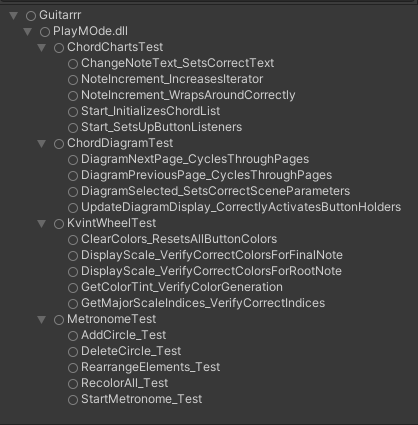
\includegraphics[scale=1]{rys05/Testy}
   \caption{Struktura testów projektu}
   \label{fig:strukturaTestów}
\end{figure}

\subsection{Implementacja testów}

Aby przeprowadzić testy dla poszczególnych komponentów, utworzono mocki (ang.~\emph{mocks} - sztuczne obiekty, udające rzeczywiste zależności). Dla tych obiektów przetestowano działanie poszczególnych funkcji.

\subsubsection{Testy metronom}

Kod przedstawiony na listingu poniżej (listing~\ref{lst:10}), odpowiada za utworzenie sztucznego obiektu \texttt{MetronomeManager}, zawierającego przyciski i pozostałe potrzebne zależności do jego działania. 

\begin{lstlisting}[style=sharpcstyle,caption=Funkcja \texttt{SetupMetronomeManager}, label=lst:10]
private MetronomeManager SetupMetronomeManager()
{
    GameObject gameObject = new GameObject();
    MetronomeManager metronomeManager = gameObject.AddComponent<MetronomeManager>();
    GameObject canvasObject = new GameObject();
    Canvas canvas = canvasObject.AddComponent<Canvas>();
    metronomeManager.canvas = canvas;
    metronomeManager.HigherTempo = CreateMockButton();
    metronomeManager.LowerTempo = CreateMockButton();
    metronomeManager.Begin = CreateMockButton();
    metronomeManager.Add = CreateMockButton();
    metronomeManager.Delete = CreateMockButton();
    ...
    return metronomeManager;
}
\end{lstlisting}

Dla klasy \texttt{MetronomeManager} sprawdzono np.\ funkcję zwiększania i zmniejszania taktu, sprawdzając przy tym, czy poprawnie tworzone są obiekty wchodzące w skład sceny (listing poniżej).

\begin{lstlisting}[style=sharpcstyle,caption=Funkcja \texttt{AddCircle\_Test}, label=lst:20]
[UnityTest]
public IEnumerator AddCircle_Test()
{
    var metronomeManager = SetupMetronomeManager();    
    metronomeManager.AddCircle();
    metronomeManager.AddCircle();
    metronomeManager.AddCircle();
    
    Assert.AreEqual(3, metronomeManager.circles.Count);
    yield return null;
}
\end{lstlisting}

Pozostałe testy obejmowały sprawdzenie poprawności funkcji odpowiedzialnych za dynamiczne rozmieszczanie elementów graficznych an scenie, działanie wątku metronomu, zmianę koloru elementów graficznych sceny, zwiększanie i zmniejszanie bpm.

\subsubsection{Testy koło kwintowe}

Testy jednostkowe koła kwintowego obejmowały utworzenie mocków obiektu głównego menadżera sceny, a następnie zbadanie działania funkcji odpowiedzialnych za zarządzanie przyciskami i elementami graficznymi scen. Na listingach ~\ref{lst:30} i \ref{lst:40} zamieszczono wybrane części kodu odpowiedzialnego za przeprowadzenie testów.

\begin{lstlisting}[style=sharpcstyle,caption=Funkcja \texttt{SetupKvintManager}, label=lst:30]
private KvintManagerScript SetupKvintManager(int outerButtonCount = 12, int innerButtonCount = 12)
{
    GameObject managerObject = new GameObject();
    KvintManagerScript kvintManager = managerObject.AddComponent<KvintManagerScript>();
    
    kvintManager.outerButtons = new List<Button>();
    for (int i = 0; i < outerButtonCount; i++)
    {
        GameObject buttonObject = new GameObject($"OuterButton_{i}");
        Button button = buttonObject.AddComponent<Button>();
        Image buttonImage = buttonObject.AddComponent<Image>();
        buttonImage.color = Color.white;
        kvintManager.outerButtons.Add(button);
    }
    return kvintManager;
}  
\end{lstlisting}

\begin{lstlisting}[style=sharpcstyle,caption=Funkcja \texttt{GetMajorScaleIndices\_VerifyCorrectIndices}, label=lst:40]
[Test]
public void GetMajorScaleIndices_VerifyCorrectIndices()
{
    var kvintManager = SetupKvintManager();
    int rootNoteIndex = 0;
    var scaleIndices = kvintManager.GetType()
        .GetMethod("GetMajorScaleIndices", System.Reflection.BindingFlags.NonPublic | System.Reflection.BindingFlags.Instance)
        .Invoke(kvintManager, new object[] { rootNoteIndex }) as List<int>;

    Assert.IsNotNull(scaleIndices);    
    List<int> expectedIndices = new List<int> { 11, 0, 1, 2, 3, 4, 5};
    CollectionAssert.AreEqual(expectedIndices, scaleIndices);
}
\end{lstlisting}

\subsubsection{Testy księga akordów}

Testy dla księgi akordów skupiały się na testowaniu działania funkcji odpowiedzialnych za zmianę aktualnie wyświetlanego akordu (listing~\ref{lst:60}). Wpierw utworzono sztuczny obiekt (listing~\ref{lst:50}), który następnie poddano testom.

\begin{lstlisting}[style=sharpcstyle,caption=Funkcja \texttt{SetupChordChartsManager}, label=lst:50]
private ChordChartsManager SetupChordChartsManager()
{

    GameObject managerObject = new GameObject();
    ChordChartsManager chordChartsManager = managerObject.AddComponent<ChordChartsManager>();

    GameObject noteTextObject = new GameObject();
    chordChartsManager.noteText = noteTextObject.AddComponent<Text>();

    GameObject variantTextObject = new GameObject();
    chordChartsManager.variantText = variantTextObject.AddComponent<Text>();

    chordChartsManager.SaveButton = CreateMockButton();
    chordChartsManager.noteLeft = CreateMockButton();
    chordChartsManager.noteRight = CreateMockButton();
    ...
    return chordChartsManager;
}
\end{lstlisting}


\begin{lstlisting}[style=sharpcstyle,caption=Funkcja \texttt{NoteIncrement\_WrapsAroundCorrectly}, label=lst:60]
[Test]
public void NoteIncrement_WrapsAroundCorrectly()
{
    var chordChartsManager = SetupChordChartsManager();
    chordChartsManager.noteIterator = 11;
    chordChartsManager.noteIncrement();
    Assert.AreEqual(0, chordChartsManager.noteIterator);

    chordChartsManager.noteDecrement();
    Assert.AreEqual(11, chordChartsManager.noteIterator);
}
\end{lstlisting}

\subsubsection{Testy diagramu akordów}

Dla głównego menadżera sceny diagramu akordów utworzono sztuczny obiekt wraz ze sztucznie utworzonymi elementami graficznymi i przyciskami, sprawdzając, czy przy przewijaniu diagramu dezaktywowane i aktywowane są odpowiednie elementy sceny. Przykłady kodu źródłowego zamieszczono na listingach (listing~\ref{lst:70}, \ref{lst:80}). Dodatkowo testowano poprawne ustawienie klasy odpowiedzialnej za komunikację pomiędzy scenami diagramu akordów i księgi akordów.

\begin{lstlisting}[style=sharpcstyle,caption=Funkcja \texttt{Setup}, label=lst:70]
[SetUp]
public void Setup()
{
    gameObject = new GameObject();
    chordDiagram = gameObject.AddComponent<ChordDiagram>();

    SetupMockComponents();
}
\end{lstlisting}

\begin{lstlisting}[style=sharpcstyle,caption=Funkcja \texttt{DiagramNextPage\_CyclesThroughPages}, label=lst:80]
[Test]
public void DiagramNextPage_CyclesThroughPages()
{
    Assert.AreEqual(0, chordDiagram.currentIndex);

    chordDiagram.DiagramNextPage();
    Assert.AreEqual(5, chordDiagram.currentIndex);

    chordDiagram.DiagramNextPage();
    Assert.AreEqual(10, chordDiagram.currentIndex);

    chordDiagram.DiagramNextPage();
    Assert.AreEqual(0, chordDiagram.currentIndex);
}
\end{lstlisting}
%\chapter{Podsumowanie}

Praca dyplomowa miała na celu utworzenie aplikacji desktopowej dla gitarzystów, służącej do nauki i doskonalenia umiejętności muzycznych. Zakres przeprowadzonych działań obejmował kompleksowy przegląd dostępnych rozwiązań, sporządzenie szczegółowych wymagań aplikacji, opracowanie projektu, implementację oraz serię testów.

Podczas wstępnej analizy przebadano dwie istniejące aplikacje, oceniając ich użyteczność i~dostępne narzędzia. Na podstawie przeprowadzonej analizy sporządzono listę kluczowych funkcji dla projektowanej aplikacji, którymi były: koło kwintowe, księga akordów, stroik gitarowy, metronom oraz trening słuchu.

Projekt został zrealizowany przy użyciu silnika Unity z wykorzystaniem języka programowania C\#. Wszystkie zaplanowane funkcje zostały poprawnie zaimplementowane i potwierdzone poprzez manualne testy aplikacji. Narzędzia umożliwiają kompleksowy trening muzyczny: metronom wspomaga ćwiczenie rytmu, księga akordów i koło kwintowe rozwijają teorię muzyczną, a trening słuchu doskonali umiejętności rozpoznawania dźwięków. Kluczowym elementem jest stroik, pozwalający na dokładne nastrojenie instrumentu.

Podczas implementacji napotkano wyzwania techniczne, zwłaszcza przy tworzeniu funkcji stroika. Wykorzystywana biblioteka analizy dźwięku wymagała modyfikacji parametrów początkowych w celu dokładnego wykrywania dźwięków. Głównym problemem było nieprawidłowe rozpoznawanie częstotliwości podstawowej, gdzie dla dźwięku A algorytm zwracał jego harmoniczne. Rozwiązaniem było ustawienie górnej granicy tolerancji, co znacząco poprawiło dokładność detekcji. Kolejnym napotkanym problemem przy realizacji funkcji stroika było zbyt duże obciążenie podczas ciągłej analizy dźwięku. Rozwiązano ten problem poprzez nagrywanie dźwięku, odtwarzanie go, gdy scena jest otwarta, a następnie wywoływanie funkcji analizy dźwięku w określonych większych odstępach czasowych. Do mniejszych problemów można zaliczyć nieprawidłowe działanie metronomu, spowodowane nieodpowiednim wywoływaniem wątku odpowiadającego za wywoływanie taktu. Ten problem udało się rozwiązać, tworząc zmienną przechowującą odwołanie do uruchomionego wątku, który był w razie potrzeby zatrzymywany i uruchamiany na nowo.

Perspektywy rozwoju aplikacji obejmują kilka potencjalnych ulepszeń takich jak: rozszerzenie funkcjonalności stroika o możliwość wyboru różnych instrumentów, wprowadzenie większej ilości skal do narzędzia treningu słuchu, implementacja dodatkowych narzędzi edukacyjnych, np. treningu pamięci muzycznej poprzez wizualne prezentowanie nut do rozpoznania, wprowadzenie zaawansowanych funkcji kompozycyjnych z wykorzystaniem algorytmów sztucznej inteligencji do automatycznego tworzenia podkładów muzycznych.

Podsumowując, projekt stanowi kompleksowe narzędzie wspierające naukę gry na gitarze, łącząc elementy praktyczne i teoretyczne, z wyraźnym potencjałem dalszego rozwoju.

% LITERATURA (zostanie wygenerowana automatycznie)
%UWAGA: bibliotekę referencji należy przygotować samemu. Dobrym do tego narzędziem jest JabRef.
%       JabRef oferuje jednak większą liczbę typów rekordów niż obsługuje BibTeX.
%       Proszę nie deklarować rekordów o typach nieobsługiwanych przez BibTeX.
%       Formatowania wykazu literatury i cytowań odbywać się ma zgodnie z zadeklarowanym stylem.
%       Zalecane są style produkujące numeryczne cytowania (w postaci [1], [2,3]).
%       Takim stylem jest np. plabbrv
\bibliographystyle{plabbrv}
%       Aby zapanować nad odstępami w wykazie literatury można posłużyć się poniższą komendą
\setlength{\bibitemsep}{2pt} % - zacieśnia wykaz
%       Pozycja Literatura pojawia się w spisie treści nieco inaczej niż spisy rysunków, tabel itp.
%       Aby zachować właściwe odstępy należy użyć poniższej komendy
\addtocontents{toc}{\addvspace{2pt}} % ustawiamy odstęp w spisie treści przed pozycją Literatura 
%       Nazwę pliku przygotowanej biblioteki wpisuje się bez rozszerzenia .bib
%       (linia poniżej załaduje rekordy z pliku "dokumentacja.bib")
\bibliography{dokumentacja}
\appendix
\chapter{Instrukcja wdrożeniowa}

Aby zainstalować aplikację na komputerze użytkownika należy uruchomić instalator(GuitarrrInstaler.exe). Instalator, jak i sama aplikacja, działają w systemie Windows 10 (i wyżej). Instalator przygotowano korzystając z narzędzia \emph{Inno Setup}. Przyjmuje ono wskazania na pliki, na podstawie których tworzy instalator aplikacji. 
% DONE: jak się nazywa instalator. Czy można go skądś pobrać? Może są jakies plany dystrubucji tej aplikacji?
Po uruchomieniu instalatora użytkownik zostanie poproszony o wybranie docelowego folderu instalacji. Jest to jedyna wymagana do ustawienia opcja. Po wykonaniu wszystkich potrzebnych procesów aplikacja znajdzie się we wskazanym przez użytkownika folderze i będzie gotowa do uruchomienia.

\chapter{Instrukcja obsługi aplikacji}

Niniejszy rozdział zawiera instrukcję obsługi dla aplikacji \emph{Guitarrr}. 

Po uruchomieniu aplikacji użytkownikowi zaprezentowane jest menu główne z 6 przyciskami:

\begin{itemize}
    \item Metronom -- po naciśnięciu użytkownik zostanie przeniesiony do widoku metronomu.
    \item Akordy gitarowe -- po naciśnięciu użytkownik zostanie przeniesiony do widoku księgi akordów.
    \item Stroik -- po naciśnięciu użytkownik zostanie przeniesiony do widoku stroika.
    \item Trening słuchu -- po naciśnięciu użytkownik zostanie przeniesiony do widoku treningu słuchu.
    \item Koło kwintowe -- po naciśnięciu użytkownik zostanie przeniesiony do widoku koła kwintowego.
    \item X -- po naciśnięciu aplikacja zostanie wyłączona.
\end{itemize}

Każdy z widoków zawiera przycisk ze znakiem "?", po naciśnięciu którego wyświetlona zostanie pomoc kontekstowa.

\subsection{Metronom}

Korzystając z metronomu, użytkownik ma dostęp do 2 przycisków odpowiedzialnych za zmianę liczby taktów (początkowo ustawione na 2) oraz 2 przyciski odpowiedzialne za zmianę liczby BPM (początkowo ustawione na 60). Aby dodać takt, należy nacisnąć przycisk z napisem "Dodaj takt", natomiast aby odjąć takt, użytkownik winien nacisnąć przycisk "Odejmij takt". Przycisk "+" służy do zwiększenia liczby BPM, natomiast "-" do ich zmniejszenia. Jeżeli użytkownik chciałby rozpocząć trening, należy nacisnąć przycisk "Start".
\subsection{Księga akordów}

Korzystając z księgi akordów na ekranie widoczny jest akord, który podpisany jest nad nim. Do zmiany akordu służą 4 przyciski, które użytkownik może naciskać, aby przeglądać listę dostępnych akordów. Poniżej akordu znajduje się przycisk "Zapisz". Po jego naciśnięciu aktualnie wyświetlany akord zostanie zapisany i będzie dostępny w widoku zapisanych akordów.
\subsection{Diagram akordów}

Diagram akordów prezentuje wszystkie dostępne w aplikacji akordy. Użytkownik może przewijać diagram za pomocą dwóch przycisków umieszczonych na dole ekranu. Po naciśnięciu na jeden z akordów użytkownik zostanie przeniesiony do widoku księgi akordów.
\subsection{Stroik}

W widoku stroika dla użytkownika dostępne jest 6 przycisków oznaczających nuty gitarowe. Po naciśnięciu jednego z przycisków rozpocznie się faza nagrywania. Wtedy użytkownik powinien wziąć swoją gitarę i uderzyć w docelową strunę. Pośrodku sceny podświetlony zostanie 1 z 3 elementów (patrząc od lewej), oznaczających: zbyt niski ton, dobry ton lub zbyt wysoki ton.
\subsection{Koło kwintowe}

Koło kwintowe zawiera 12 przycisków zewnętrznych, z którymi użytkownik może wchodzić w~interakcję. Po naciśnięciu jednego z przycisków na zewnętrznym kole, kolorowo zaznaczone zostaną te nuty, które wchodzą w skład skali majorowej, dla której wybrana nuta jest tonem głównym. Ponadto na szaro podświetlą się przyciski symbolizujące akordy pasujące do danej skali.
\subsection{Trening słuchu}

Scena treningu słuchu wita użytkownika wyborem 4 możliwych tonacji do odbycia treningu. Po wybraniu jednej z 4 możliwych tonacji przed użytkownikiem pojawi się odpowiadająca skala majorowa. Następnie należy nacisnąć przycisk "GRAJ", po czym odgadnąć odegraną nutę za pomocą dostępnych przycisków. W razie chęci zmiany skali należy nacisnąć przycisk reset. Po jego naciśnięciu ponownie wyświetlone zostaną 4 możliwe tonacje.


% Jeśli w pracy pojawiać się ma indeks, należy odkomentować poniższe linie
%%\chapterstyle{noNumbered}
%%\phantomsection % sets an anchor
%%\addcontentsline{toc}{chapter}{Indeks rzeczowy}
%%\printindex

\end{document}
